\begin{name}
	{\tenchude}{\tendethi}{LỚP TOÁN THẦY PHÁT}{\thoigian}
\end{name}
\setcounter{ex}{0}\setcounter{bt}{0}
\Opensolutionfile{ans}[ans/ans-2-TT-12-KienThuy-HaiPhong-23]

\begin{ex}%[Đề thi thử THPT Kiến Thuỵ - Thái Bình]%[Bùi Mạnh Tiến, dự án 12EX-6]%[2H3Y3-2]
	Trong không gian $Oxyz$, phương trình của đường thẳng đi qua điểm $A(1;2;-1)$ và có véc-tơ chỉ phương $\overrightarrow{u}=(1;3;2)$ là
	\choice
	{$\dfrac{x+1}{1}=\dfrac{y+3}{2}=\dfrac{z+2}{-1}$}
	{$\dfrac{x-1}{1}=\dfrac{y-3}{2}=\dfrac{z-2}{-1}$}
	{$\dfrac{x+1}{1}=\dfrac{y+2}{3}=\dfrac{z-1}{2}$}
	{\True $\dfrac{x-1}{1}=\dfrac{y-2}{3}=\dfrac{z+1}{2}$}
	\loigiai
	{
		Đường thẳng đi qua $A(1;2;-1)$ và có véc-tơ chỉ phương $\overrightarrow{u}=(1;3;2)$ có phương trình là
		\begin{align*}
			\dfrac{x-1}{1}=\dfrac{y-2}{3}=\dfrac{z+1}{2}.
		\end{align*}	
	}
\end{ex}

\begin{ex}%[Đề thi thử THPT Kiến Thuỵ - Thái Bình]%[Bùi Mạnh Tiến, dự án 12EX-6]%[2D2Y4-1]
	Tập xác định của hàm số $y=\log_2 (x-3)$ là
	\choice
	{$(-\infty;3)$}
	{\True $(3;+\infty)$}
	{$\mathbb{R}\setminus \{3\}$}
	{$\left[3;+\infty\right)$}
	\loigiai
	{
		Điều kiện xác định: $x-3>0\Leftrightarrow x>3$.\\
		Tập xác định của hàm số là $\mathscr{D}=(3;+\infty)$.
	}
\end{ex}

\begin{ex}%[Đề thi thử THPT Kiến Thuỵ - Thái Bình]%[Bùi Mạnh Tiến, dự án 12EX-6]%[2D2Y3-2]
	Cho $a$ là số thực dương khác $1$ và $x$, $y$ là các số thực dương. Mệnh đề nào dưới đây đúng?
	\choice
	{$\log_a \dfrac{x}{y}=\dfrac{\log_a x}{\log_a y}$}
	{\True $\log_a \dfrac{x}{y}=\log_a x-\log_a y$}
	{$\log_a \dfrac{x}{y}=\log_a (x-y)$}
	{$\log_a \dfrac{x}{y}=\log_a y-\log_a x$}
	\loigiai
	{
		Với $a$ là số thực dương khác $1$ và $x$, $y$ là các số thực dương ta có $\log_a \dfrac{x}{y}=\log_a x-\log_a y$.
	}
\end{ex}

\begin{ex}%[Đề thi thử THPT Kiến Thuỵ - Thái Bình]%[Bùi Mạnh Tiến, dự án 12EX-6]%[1D3Y4-3]
	Cho cấp số nhân $(u_n)$ với $u_1=2$ và công bội $q=3$. Giá trị của $u_2$ là
	\choice
	{$8$}
	{$\dfrac{2}{3}$}
	{\True $6$}
	{$9$}
	\loigiai
	{
		Cấp số nhân $(u_n)$ có $u_2=u_1\cdot q=2\cdot 3=6$.	
	}
\end{ex}

\begin{ex}%[Đề thi thử THPT Kiến Thuỵ - Thái Bình]%[Bùi Mạnh Tiến, dự án 12EX-6]%[2H1Y3-2]
	Thể tích của khối chóp có đáy là hình vuông cạnh bằng $2$ và chiều cao bằng $6$ là
	\choice
	{\True $8$}
	{$12$}
	{$24$}
	{$4$}
	\loigiai
	{
		Thể tích khối chóp có đáy là hình vuông cạnh bằng $a=2$ và chiều cao bằng $h=6$	là
		\begin{align*}
			V=\dfrac{1}{3}S\cdot h=\dfrac{1}{3}a^2\cdot h=\dfrac{1}{3}\cdot 2^2\cdot 6=8.
		\end{align*}	
	}
\end{ex}

\begin{ex}%[Đề thi thử THPT Kiến Thuỵ - Thái Bình]%[Bùi Mạnh Tiến, dự án 12EX-6]%[2D3Y1-2]
	Cho hàm số $f(x)=\mathrm{e}^{2x}$. Khẳng định nào sau đây đúng?
	\choice
	{$\displaystyle\int f(x) \mathrm{\,d}x=\mathrm{e}^{2x}+C$}
	{$\displaystyle\int f(x) \mathrm{\,d}x=2\mathrm{e}^{2x}+C$}
	{\True $\displaystyle\int f(x) \mathrm{\,d}x=\dfrac{1}{2}\mathrm{e}^{2x}+C$}
	{$\displaystyle\int f(x) \mathrm{\,d}x=\dfrac{\mathrm{e}^{2x+1}}{2x+1}+C$}
	\loigiai
	{
		Ta có $\displaystyle\int f(x) \mathrm{\,d}x=\dfrac{1}{2}\displaystyle\int \mathrm{e}^{2x} \mathrm{\,d}(2x)=\dfrac{1}{2}\mathrm{e}^{2x}+C$.
	}
\end{ex}

\begin{ex}%[Đề thi thử THPT Kiến Thuỵ - Thái Bình]%[Bùi Mạnh Tiến, dự án 12EX-6]%[2D1Y2-2]
	\immini
	{
		Cho hàm số $y=f(x)$ có đồ thị là đường cong trong hình vẽ bên. Giá trị cực đại của hàm số đã cho bằng
		\choice
		{$1$}
		{$0$}
		{\True $4$}
		{$-1$}
	}
	{
		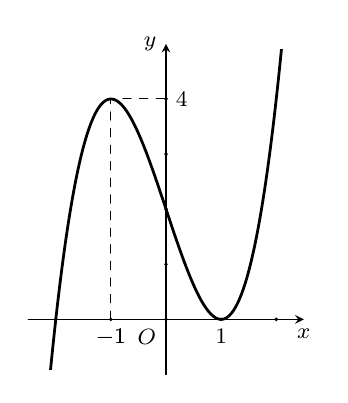
\begin{tikzpicture}[line join = round, line cap = round,>=stealth,font=\footnotesize,scale=0.7]
			\def \xmin{-2.5};
			\def \xmax{2.5};
			\def \ymin{-1};
			\def \ymax{5};
			\draw[->] (\xmin,0) -- (\xmax,0) node[below] {$x$};
			\draw[->] (0,\ymin) -- (0,0) node[below left] {$O$} -- (0,\ymax) node[left] {$y$};
			\clip (\xmin+0.1,\ymin+0.1) rectangle (\xmax-0.1,\ymax-0.1);
			\draw[smooth, line width=1,samples=100] plot[domain=-2.3:2.3] (\x,{(\x)^3-3*(\x)+2});
			\draw[dashed] (-1,0) node[below] {$-1$} -- (-1,4) -- (0,4) node[right] {$4$};
			\foreach \y in {0,1,...,4}
			{
				\fill (0,\y) circle (1pt);
			}
			\foreach \x in {-2,-1,1,2}
			{
				\fill (\x,0) circle (1pt);
			}
			\draw (-1,0) node[below] {$-1$};
			\draw (1,0) node[below] {$1$};
		\end{tikzpicture}
	}
	\loigiai
	{
		Dựa vào đồ thị hàm số trên ta thấy rằng hàm số có giá trị cực đại $y=4$ tại điểm $x=-1$.
	}
\end{ex}

\begin{ex}%[Đề thi thử THPT Kiến Thuỵ - Thái Bình]%[Bùi Mạnh Tiến, dự án 12EX-6]%[2D1Y1-2]
	Cho hàm số $y=f(x)$ có bảng biến thiên như sau
	\begin{center}
		
\begin{tikzpicture}[line join = round, line cap = round,>=stealth,font=\footnotesize,scale=1]
			\tkzTabInit[nocadre=false,lgt=1.2,espcl=2.5,deltacl=0.6]
			{$x$ /0.6, $f’(x)$ /0.6, $f(x)$ /2}
			{$-\infty$,$-1$,$0$,$1$,$+\infty$}
			\tkzTabLine{ ,-,z,+,z,-,z,+, }
			\tkzTabVar{+/$+\infty$,-/$-2$,+/$3$,-/$-2$,+/$+\infty$}
		\end{tikzpicture}
	\end{center}
	Hàm số đã cho nghịch biến trên khoảng nào dưới đây?
	\choice
	{$(1;+\infty)$}
	{\True $(-\infty;-1)$}
	{$(-1;0)$}
	{$(-2;3)$}
	\loigiai
	{
		Dựa vào bảng biến thiên ở hình trên ta thấy hàm số đã cho nghịch biến trên các khoảng $(-\infty;-1)$ và $(0;1)$.
	}
\end{ex}

\begin{ex}%[Đề thi thử THPT Kiến Thuỵ - Thái Bình]%[Bùi Mạnh Tiến, dự án 12EX-6]%[2D1Y4-1]
	Tiệm cận ngang của đồ thị hàm số $y=\dfrac{2x+3}{x-1}$ là đường thẳng có phương trình
	\choice
	{$y=1$}
	{$y=-2$}
	{$y=-1$}
	{\True $y=2$}
	\loigiai
	{
		Vì $\lim \limits_{x \to +\infty} \dfrac{2x+3}{x-1}=\lim \limits_{x \to +\infty}\dfrac{2+\dfrac{3}{x}}{1-\dfrac{1}{x}}=2$ và $\lim \limits_{x \to -\infty} \dfrac{2x+3}{x-1}=\lim \limits_{x \to -\infty}\dfrac{2+\dfrac{3}{x}}{1-\dfrac{1}{x}}=2$ nên $y=2$ là tiệm cận ngang của đồ thị hàm số.	
	}
\end{ex}

\begin{ex}%[Đề thi thử THPT Kiến Thuỵ - Thái Bình]%[Bùi Mạnh Tiến, dự án 12EX-6]%[2D1Y1-1]
	Hàm số $y=2x^3-2x^2-2x+1$ đồng biến trên khoảng nào dưới đây?
	\choice
	{$(-1;1)$}
	{$(-\infty;1)$}
	{$(0;2)$}
	{\True $(1;2)$}
	\loigiai
	{
		Ta có $y'=6x^2-4x-2$, $y'=0\Leftrightarrow 6x^2-4x-2=0\Leftrightarrow \hoac{& x=1 \\ & x=-\dfrac{1}{3}.}$\\
		Ta có bảng xét dấu của hàm số $f'(x)$ như sau
		\begin{center}
			
\begin{tikzpicture}[line join = round, line cap = round,>=stealth,font=\footnotesize,scale=1]
				\tkzTabInit[nocadre=false,lgt=1.2,espcl=2.5,deltacl=0.6]
				{$x$ /0.6, $f’(x)$ /0.6}
				{$-\infty$,$-\frac{1}{3}$,$1$,$+\infty$}
				\tkzTabLine{ ,+,z,-,z,+, }
			\end{tikzpicture}
		\end{center}
		Dựa vào bảng xét dấu của $f'(x)$ ta thấy hàm số đồng biến trên các khoảng $\left(-\infty;-\dfrac{1}{3}\right)$ và $(1;+\infty)\Rightarrow$ hàm số cũng đồng biến trên $(1;2)$.
	}
\end{ex}

\begin{ex}%[Đề thi thử THPT Kiến Thuỵ - Thái Bình]%[Bùi Mạnh Tiến, dự án 12EX-6]%[2D1Y5-1]
	\immini
	{
		Đường cong trong hình bên là đồ thị của hàm số nào dưới đây?
		\choice
		{$y=x^4-3x^2-2$}
		{$y=-x^4+3x^2-2$}
		{$y=-x^3-3x^2-2$}
		{\True $y=x^3+3x^2-2$}
	}
	{
		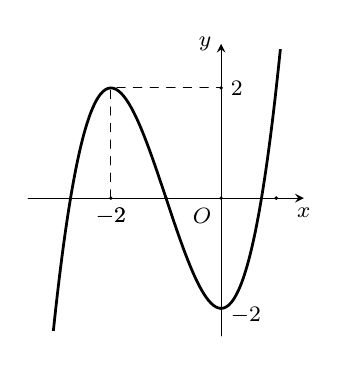
\begin{tikzpicture}[line join = round, line cap = round,>=stealth,font=\footnotesize,scale=0.7]
			\def \xmin{-3.5};
			\def \xmax{1.5};
			\def \ymin{-2.5};
			\def \ymax{2.8};
			\draw[->] (\xmin,0) -- (\xmax,0) node[below] {$x$};
			\draw[->] (0,\ymin) -- (0,0) node[below left] {$O$} -- (0,\ymax) node[left] {$y$};
			\clip (\xmin+0.1,\ymin+0.1) rectangle (\xmax-0.1,\ymax-0.1);
			\draw[smooth, line width=1,samples=100] plot[domain=-3.3:1.3] (\x,{(\x)^3+3*(\x)^2-2});
			\draw[dashed] (-2,0) node[below] {$-2$} -- (-2,2) -- (0,2) node[right] {$2$};
			\foreach \y in {-2,2}
			{
				\fill (0,\y) circle (1pt);
			}
			\foreach \x in {-2,-1,1,0}
			{
				\fill (\x,0) circle (1pt);
			}
			\draw (-2,0) node[below] {$-2$};
			\draw (0,-1.8) node[below right] {$-2$};
		\end{tikzpicture}
	}
	\loigiai
	{
		Đồ thị hình trên cho ta thấy đây là đồ thị hàm số bậc ba với hệ số của $x^3$ là hệ số dương.
	}
\end{ex}

\begin{ex}%[Đề thi thử THPT Kiến Thuỵ - Thái Bình]%[Bùi Mạnh Tiến, dự án 12EX-6]%[2D4Y1-1]
	Số phức liên hợp của số phức $z=6-4i$ là
	\choice
	{$\overline{z}=-6-4i$}
	{$\overline{z}=-6+4i$}
	{\True $\overline{z}=6+4i$}
	{$\overline{z}=6-4i$}
	\loigiai
	{
		Số phức liên hợp của số phức $z=6-4i$ là $\overline{z}=6+4i$.
	}
\end{ex}

\begin{ex}%[Đề thi thử THPT Kiến Thuỵ - Thái Bình]%[Bùi Mạnh Tiến, dự án 12EX-6]%[2D3Y2-1]
	Nếu $\displaystyle\int\limits_{3}^{4} f(x) \mathrm{\,d}x=3$ thì $\displaystyle\int\limits_{3}^{4} -4f(x) \mathrm{\,d}x$ bằng
	\choice
	{\True $-12$}
	{$4$}
	{$12$}
	{$3$}
	\loigiai
	{
		Ta có $\displaystyle\int\limits_{3}^{4} -4f(x) \mathrm{\,d}x=-4\displaystyle\int\limits_{3}^{4} f(x) \mathrm{\,d}x=(-4)\cdot 3=-12$.
	}
\end{ex}

\begin{ex}%[Đề thi thử THPT Kiến Thuỵ - Thái Bình]%[Bùi Mạnh Tiến, dự án 12EX-6]%[2H2Y2-1]
	Cho khối cầu có bán kính $R$. Thể tích của khối cầu đó là
	\choice
	{$V=4\pi R^3$}
	{\True $V=\dfrac{4}{3}\pi R^3$}
	{$V=\dfrac{1}{3}\pi R^3$}
	{$V=\dfrac{4}{3}\pi R^2$}
	\loigiai
	{
		Thể tích của khối cầu có bán kính $R$ là $V=\dfrac{4}{3}\pi R^3$.	
	}
\end{ex}

\begin{ex}%[Đề thi thử THPT Kiến Thuỵ - Thái Bình]%[Bùi Mạnh Tiến, dự án 12EX-6]%[2H3Y1-3]
	Trong không gian với hệ tọa độ $Oxyz$, tọa độ tâm $I$ và bán kính $R$ của mặt cầu có phương trình $(x+2)^2+(y-3)^2+z^2=5$ là
	\choice
	{$I(2;-3;0)$, $R=5$}
	{$I(-2;3;0)$, $R=5$}
	{\True $I(-2;3;0)$, $R=\sqrt{5}$}
	{$I(2;-3;0)$, $R=\sqrt{5}$}
	\loigiai
	{
		Mặt cầu có phương trình $(x+2)^2+(y-3)^2+z^2=5$ có tâm $I(-2;3;0)$ và bán kính $R=\sqrt{5}$.
	}
\end{ex}

\begin{ex}%[Đề thi thử THPT Kiến Thuỵ - Thái Bình]%[Bùi Mạnh Tiến, dự án 12EX-6]%[2H3Y2-4]
	Trong không gian $Oxyz$, cho mặt phẳng $(\alpha)\colon x-2y+2z-3=0$. Điểm nào sau đây nằm trên mặt phẳng $(\alpha)$?
	\choice
	{$M(2;0;1)$}
	{$Q(2;1;1)$}
	{$P(2;-1;1)$}
	{\True $N(1;0;1)$}
	\loigiai
	{
		Ta thấy $1-2\cdot 0+2\cdot 1-3=0\Rightarrow N(1;0;1)$ nằm trên mặt phẳng $(\alpha)$.
	}
\end{ex}

\begin{ex}%[Đề thi thử THPT Kiến Thuỵ - Thái Bình]%[Bùi Mạnh Tiến, dự án 12EX-6]%[2D4B2-4]
	Trên mặt phẳng toạ độ $Oxy$, tập hợp điểm biểu diễn các số phức $z$ thoả mãn điều kiện $|z-1+2i|=3$ là đường tròn có toạ độ tâm là
	\choice
	{$(2;-1)$}
	{$(1;2)$}
	{\True $(1;-2)$}
	{$(-1;-2)$}
	\loigiai
	{
		Gọi $M(x;y)$ là điểm biểu diễn số phức $z=x+yi$ (với $x$, $y\in \mathbb{R}$). Ta có
		\begin{eqnarray*}
			|z-1+2i|=3&\Leftrightarrow &|x+yi-1+2i|=3\\
			&\Leftrightarrow &|(x-1)+(y+2)i|=3\\
			&\Leftrightarrow &\sqrt{(x-1)^2+(y+2)^2}=3\\
			&\Leftrightarrow &(x-1)^2+(y+2)^2=9.
		\end{eqnarray*}
		Vậy tập hợp điểm $M$ biểu diễn số phức $z$ là đường tròn tâm $I(1;-2)$ và có bán kính $R=3$.
	}
\end{ex}

\begin{ex}%[Đề thi thử THPT Kiến Thuỵ - Thái Bình]%[Bùi Mạnh Tiến, dự án 12EX-6]%[2D2B6-1]
	Tập nghiệm $S$ của bất phương trình $\log_{\frac{1}{2}}(x+1)<\log_{\frac{1}{2}}(2x-1)$ là
	\choice
	{\True $S=\left(\dfrac{1}{2};2\right)$}
	{$S=(-1;2)$}
	{$S=(-\infty;2)$}
	{$S=(2;+\infty)$}
	\loigiai
	{
		Ta có $\log_{\frac{1}{2}}(x+1)<\log_{\frac{1}{2}}(2x-1)\Leftrightarrow 0<2x-1<x+1\Leftrightarrow \heva{& x>\dfrac{1}{2} \\ & x<2}\Leftrightarrow \dfrac{1}{2}<x<2$.\\
		Vậy tập nghiệm của bất phương trình là $S=\left(\dfrac{1}{2};2\right)$.
	}
\end{ex}

\begin{ex}%[Đề thi thử THPT Kiến Thuỵ - Thái Bình]%[Bùi Mạnh Tiến, dự án 12EX-6]%[2H3B1-1]
	Trong không gian với hệ tọa độ $Oxyz$, cho tứ diện $ABCD$ với $A(1;-4;2)$, $B(2;1;-3)$, $C(3;0;-2)$ và $D(2;-5;-1)$. Điểm $G$ thoả mãn $\overrightarrow{GA}+\overrightarrow{GB}+\overrightarrow{GC}+\overrightarrow{GD}=\overrightarrow{0}$ có toạ độ là
	\choice
	{$G(2;-1;-1)$}
	{\True $G(2;-2;-1)$}
	{$G(0;-1;-1)$}
	{$G(6;-3;-3)$}
	\loigiai
	{
		Ta có $\overrightarrow{GA}+\overrightarrow{GB}+\overrightarrow{GC}+\overrightarrow{GD}=\overrightarrow{0}\Leftrightarrow \overrightarrow{OA}-\overrightarrow{OG}+\overrightarrow{OB}-\overrightarrow{OG}+\overrightarrow{OC}-\overrightarrow{OG}+\overrightarrow{OD}-\overrightarrow{OG}=\overrightarrow{0}\Leftrightarrow \overrightarrow{OG}=\dfrac{1}{4}\left(\overrightarrow{OA}+\overrightarrow{OB}+\overrightarrow{OC}+\overrightarrow{OD}\right)$.\\
		Suy ra $\heva{& x_G=\dfrac{x_A+x_B+x_C+x_D}{4}=\dfrac{1+2+3+2}{4}=2\\ & y_G=\dfrac{y_A+y_B+y_C+y_D}{4}=\dfrac{-4+1+0-5}{4}=-2\\& z_G=\dfrac{z_A+z_B+z_C+z_D}{4}=\dfrac{2-3-2-1}{4}=-1}\Rightarrow G(2;-2;-1)$.
	}
\end{ex}

\begin{ex}%[Đề thi thử THPT Kiến Thuỵ - Thái Bình]%[Bùi Mạnh Tiến, dự án 12EX-6]%[2D2B6-1]
	Số nghiệm nguyên của bất phương trình $\left(\dfrac{1}{5}\right)^{-3x^2}<5^{5x+2}$ là
	\choice
	{$3$}
	{$1$}
	{\True $2$}
	{$4$}
	\loigiai
	{
		Ta có $\left(\dfrac{1}{5}\right)^{-3x^2}<5^{5x+2}\Leftrightarrow 5^{3x^2}<5^{5x+2}\Leftrightarrow 3x^2<5x+2\Leftrightarrow 3x^2-5x-2<0\Leftrightarrow -\dfrac{1}{3}<x<2$.\\
		Vì $x$ là số nguyên dương nên $x\in \{0;1\}$.\\
		Có tất cả $2$ giá trị nguyên dương của $x$ thoả mãn yêu cầu bài toán.
	}
\end{ex}

\begin{ex}%[Đề thi thử THPT Kiến Thuỵ - Thái Bình]%[Bùi Mạnh Tiến, dự án 12EX-6]%[1D2B2-1]
	Có bao nhiêu cách xếp $5$ quyển sách Văn và $7$ sách quyển Toán khác nhau trên một kệ sách dài sao cho các quyển sách Văn phải xếp kề nhau?
	\choice
	{\True $5!\cdot 8!$}
	{$5!\cdot 7!$}
	{$2\cdot 5!\cdot 7!$}
	{$12!$}
	\loigiai
	{
		Ta coi $5$ quyển sách văn là $1$ phần tử $V$. Xếp $7$ quyển sách Toán và phần tử $V$ có $8!$ cách xếp.\\
		Đổi chỗ $5$ quyển sách Văn ta có $5!$ cách xếp.\\
		Số cách xếp $5$ quyển sách Văn và $7$ quyển sách Toán khác nhau trên một kệ dài sao cho $5$ quyển sách Văn xếp kề nhau là $8!\cdot 5!$ cách xếp. 
	}
\end{ex}

\begin{ex}%[Đề thi thử THPT Kiến Thuỵ - Thái Bình]%[Bùi Mạnh Tiến, dự án 12EX-6]%[2H1B3-3]
	Cho khối lăng trụ $ABC.A'B'C'$ có thể tích bằng $15$. Thể tích của khối chóp $A'.ABC$ bằng
	\choice
	{$3$}
	{$10$}
	{\True $5$}
	{$6$}
	\loigiai
	{
		Ta có $V_{A'.ABC}=\dfrac{1}{3}\mathrm{d}(A',(ABC))\cdot S_{ABC}=\dfrac{1}{3}V_{A'B'C'.ABC}=\dfrac{1}{3}\cdot 15=5$.	
	}
\end{ex}

\begin{ex}%[Đề thi thử THPT Kiến Thuỵ - Thái Bình]%[Bùi Mạnh Tiến, dự án 12EX-6]%[2D4B2-3]
	Biết $z=a+bi$ ($a$, $b\in \mathbb{R}$) là số phức thoả mãn $(3-2i)z-2i\overline{z}=15-8i$. Tổng $2a+b$ là
	\choice
	{$2a+b=5$}
	{\True $2a+b=14$}
	{$2a+b=9$}
	{$2a+b=12$}
	\loigiai
	{
		Ta có $z=a+bi\Rightarrow \overline{z}=a-bi$. Ta có
		\begin{eqnarray*}
			(3-2i)z-2i\overline{z}=15-8i&\Leftrightarrow & (3-2i)(a+bi)-2i(a-bi)=15-8i\\
			&\Leftrightarrow & 3a+2b+(-2a+3b)i-2ai-2b=15-8i\\
			&\Leftrightarrow & 3a+(3b-4a)i=15-8i\\
			&\Leftrightarrow & \heva{& 3a=15 \\ & 3b-4a=-8}\\
			&\Leftrightarrow &\heva{& a=5 \\ & b=4.}
		\end{eqnarray*}
		Vậy $2a+b=2\cdot 5+4=14$.
	}
\end{ex}

\begin{ex}%[Đề thi thử THPT Kiến Thuỵ - Thái Bình]%[Bùi Mạnh Tiến, dự án 12EX-6]%[2H3B2-2]
	Trong không gian với hệ tọa độ $Oxyz$, cho ba điểm $A(1;-2;1)$, $B(-1;3;3)$, $C(2;-4;2)$. Một véc-tơ pháp tuyến $\overrightarrow{n}$ của mặt phẳng $(ABC)$ là
	\choice
	{$\overrightarrow{n}=(-1;9;4)$}
	{$\overrightarrow{n}=(9;4;1)$}
	{$\overrightarrow{n}=(4;9;-1)$}
	{\True $\overrightarrow{n}=(9;4;-1)$}
	\loigiai
	{
		Ta có $\overrightarrow{AB}=(-2;5;2)$, $\overrightarrow{AC}=(1;-2;1)$.\\
		Mặt phẳng $(ABC)$ nhận $\overrightarrow{n}=\left[\overrightarrow{AB},\overrightarrow{AC}\right]=(9;4;-1)$ làm một véc-tơ pháp tuyến.
	}
\end{ex}

\begin{ex}%[Đề thi thử THPT Kiến Thuỵ - Thái Bình]%[Bùi Mạnh Tiến, dự án 12EX-6]%[2D2B5-1]
	Tích tất cả các nghiệm của phương trình $2^{2x^2+5x+4}=4$ bằng
	\choice
	{\True $1$}
	{$-2$}
	{$2$}
	{$-1$}
	\loigiai
	{
		Ta có $2^{2x^2+5x+4}=4\Leftrightarrow 2^{2x^2+5x+4}=2^2\Leftrightarrow 2x^2+5x+4=2\Leftrightarrow 2x^2+5x+2=0\Leftrightarrow \hoac{& x=-2 \\ & x=-\dfrac{1}{2}.}$\\
		Tích tất cả các nghiệm của phương trình đã cho là $\left(-2\right)\cdot \left(-\dfrac{1}{2}\right)=1$.
	}
\end{ex}

\begin{ex}%[Đề thi thử THPT Kiến Thuỵ - Thái Bình]%[Bùi Mạnh Tiến, dự án 12EX-6]%[2H3B2-4]
	Trong không gian $Oxyz$, cho đường thẳng $d\colon \heva{& x=1+2t \\ & y=3-t\\& z=1-t}$, $t\in \mathbb{R}$ và mặt phẳng $(P)\colon x+2y-3z+2=0$. Toạ độ của giao điểm $A$ của đường thẳng $d$ và mặt phẳng $(P)$ là
	\choice
	{$A(3;5;3)$}
	{$A(1;3;1)$}
	{\True $A(-3;5;3)$}
	{$A(1;2;-3)$}
	\loigiai
	{
		Vì $A\in d\Rightarrow A(1+2t;3-t;1-t)$. Mà $A\in (P)$ nên
		\begin{align*}
			1+2t+2(3-t)-3(1-t)+2=0\Leftrightarrow 3t+6=0\Leftrightarrow t=-2\Rightarrow A(-3;5;3).
		\end{align*}
	}
\end{ex}

\begin{ex}%[Đề thi thử THPT Kiến Thuỵ - Thái Bình]%[Bùi Mạnh Tiến, dự án 12EX-6]%[2H2B1-1]
	Một hình nón có đường sinh bằng $2a$ và góc giữa đường sinh và mặt phẳng đáy bằng $60^\circ$. Thể tích của khối nón được tạo nên từ hình nón đã cho bằng
	\choice
	{\True $\dfrac{\sqrt{3}}{3}\pi a^3$}
	{$\dfrac{\sqrt{3}}{324}\pi a^3$}
	{$\pi a^3$}
	{$4\pi a^3$}
	\loigiai
	{
		\immini
		{
			Vì góc giữa đường sinh và mặt phẳng đáy là $60^\circ\Rightarrow \widehat{SBO}=60^\circ$. Ta có
			\begin{align*}
				\cos \widehat{SBO}=\dfrac{BO}{BS}\Leftrightarrow \cos 60^\circ=\dfrac{r}{\ell}\Leftrightarrow r=\ell \cos 60^\circ=2a\cdot \cos 60^\circ=a.
			\end{align*}
			Khi đó chiều cao của khối nón là $h=\sqrt{\ell ^2-r^2}=\sqrt{(2a)^2-a^2}=a\sqrt{3}$.\\
			Thể tích của khối nón là $V=\dfrac{1}{3}\pi r^2\cdot h=\dfrac{\sqrt{3}}{3}\pi a^3$.	
		}
		{
			\begin{tikzpicture}[line join = round, line cap = round,>=stealth,font=\footnotesize,scale=1]	\def \x{1.5}  %bán kính trục lớn elip
				\def \y{0.4}  %bán kính trục bé elip
				\def \h{2.5}  %chiều cao hình nón
				\coordinate (A) at (0,0);
				\coordinate (B) at (2*\x,0);
				\coordinate (O) at ($(A)!0.5!(B)$);
				\coordinate (S) at ($(O)+(0,\h)$);
				\draw[dashed] (B) arc (0:180:\x cm and \y cm);
				\draw (B) arc (0:-180:\x cm and \y cm);
				\draw (B) -- (S) -- (A);
				\draw[dashed] (A) -- (B) (S) -- (O);
				\foreach \x/\g in {A/180,B/0,O/-90,S/90} \fill[black](\x) circle (1pt)+(\g:3mm) node{$\x$};
				\path 
				(S) -- (B) node[right,pos=0.5] {$\ell$}
				(S) -- (O) node[right,pos=0.5] {$h$}
				(O) -- (B) node[below,pos=0.5] {$r$}
				;
				\tkzMarkAngles[size=0.8cm,arc=l,mark=](S,B,O)
				\draw ($(B)+(-0.4,0.2)$) node {$60^\circ$};
			\end{tikzpicture}
			
		}
	}
\end{ex}

\begin{ex}%[Đề thi thử THPT Kiến Thuỵ - Thái Bình]%[Bùi Mạnh Tiến, dự án 12EX-6]%[2D3B3-3]
	Cho hình phẳng $D$ giới hạn bởi các đường $y=\sqrt{x-1}$, trục hoành và $x=5$. Thể tích khối tròn xoay tạo thành khi quay $D$ xung quanh trục $Ox$ bằng
	\choice
	{$\dfrac{15\pi}{2}$}
	{$\dfrac{15}{2}$}
	{\True $8\pi$}
	{$8$}
	\loigiai
	{
		Hoành độ giao điểm của đường cong $y=\sqrt{x-1}$ và trục hoành là nghiệm của phương trình $\sqrt{x-1}=0\Leftrightarrow x=1$.\\
		Thể tích khối tròn xoay khi $D$ quay quanh trục $Ox$ là
		\begin{align*}
			V=\pi \displaystyle\int\limits_{1}^{5} \left(\sqrt{x-1}\right)^2 \mathrm{\,d}x=\pi \displaystyle\int\limits_{1}^{5} (x-1) \mathrm{\,d}x=\pi \left(\dfrac{x^2}{2}-x\right)\bigg|_{1}^5=8\pi.
		\end{align*}	
	}
\end{ex}

\begin{ex}%[Đề thi thử THPT Kiến Thuỵ - Thái Bình]%[Bùi Mạnh Tiến, dự án 12EX-6]%[2D3B3-1]
	\immini
	{
		Cho hàm số $f(x)$ liên tục trên $\mathbb{R}$. Gọi $S$ là diện tích hình phẳng giới hạn bởi các đường $y=f(x)$, $y=0$, $x=-1$, $x=2$ (như hình vẽ bên). Mệnh đề nào dưới đây đúng?
		\choice
		{$S=\displaystyle\int\limits_{-1}^{1} f(x) \mathrm{\,d}x+\displaystyle\int\limits_{1}^{2} f(x) \mathrm{\,d}x$}
		{\True $S=\displaystyle\int\limits_{-1}^{1} f(x) \mathrm{\,d}x-\displaystyle\int\limits_{1}^{2} f(x) \mathrm{\,d}x$}
		{$S=-\displaystyle\int\limits_{-1}^{1} f(x) \mathrm{\,d}x-\displaystyle\int\limits_{1}^{2} f(x) \mathrm{\,d}x$}
		{$S=-\displaystyle\int\limits_{-1}^{1} f(x) \mathrm{\,d}x+\displaystyle\int\limits_{1}^{2} f(x) \mathrm{\,d}x$}
	}
	{
		\begin{tikzpicture}[line join = round, line cap = round,>=stealth,font=\footnotesize,scale=0.8]
			\def \xmin{-2};
			\def \xmax{3};
			\def \ymin{-1.2};
			\def \ymax{3.2};
			\draw[->] (\xmin,0) -- (\xmax,0) node[below] {$x$};
			\draw[->] (0,\ymin) -- (0,0) node[below left] {$O$} -- (0,\ymax) node[left] {$y$};
			\clip (\xmin+0.1,\ymin+0.1) rectangle (\xmax-0.1,\ymax-0.1);
			\draw[smooth, line width=1,samples=100] plot[domain=-1.5:2.5] (\x,{1.25*(\x+1)*(\x-1)*(\x-2)});
			\draw[smooth, line width=1,samples=100,pattern=north east lines] plot[domain=-1:2] (\x,{1.25*(\x+1)*(\x-1)*(\x-2)});
			\foreach \x in {-1,1,2}
			{
				\fill (\x,0) circle (1pt);
			}
			\draw (-1,0) node[below left] {$-1$};
			\draw (1,0) node[below left] {$1$};
			\draw (2,0) node[below right] {$2$}; 
		\end{tikzpicture}
	}
	\loigiai
	{
		Diện tích hình phẳng giới hạn bởi các đường $y=f(x)$, $y=0$, $x=-1$, $x=2$ là
		\begin{align*}
			S=\displaystyle\int\limits_{-1}^{2} |f(x)| \mathrm{\,d}x=\displaystyle\int\limits_{-1}^{1} |f(x)| \mathrm{\,d}x+\displaystyle\int\limits_{1}^{2} |f(x)| \mathrm{\,d}x=\displaystyle\int\limits_{-1}^{1} f(x) \mathrm{\,d}x-\displaystyle\int\limits_{1}^{2} f(x) \mathrm{\,d}x.
		\end{align*}
	}
\end{ex}

\begin{ex}%[Đề thi thử THPT Kiến Thuỵ - Thái Bình]%[Bùi Mạnh Tiến, dự án 12EX-6]%[2D1B2-1]
	Cho hàm số $y=f(x)$ có đạo hàm $f'(x)=2x(x-2)(x+3)^5$, $\forall x\in \mathbb{R}$. Số điểm cực tiểu của hàm số đã cho là
	\choice
	{$1$}
	{\True $2$}
	{$3$}
	{$0$}
	\loigiai
	{
		Ta có $f'(x)=0\Leftrightarrow 2x(x-2)(x+3)^5=0\Leftrightarrow \hoac{& x=0 \\ & x=2\\& x=-3.}$\\
		Bảng xét dấu của hàm số $f'(x)$ là
		\begin{center}
			
\begin{tikzpicture}[line join = round, line cap = round,>=stealth,font=\footnotesize,scale=1]
				\tkzTabInit[nocadre=false,lgt=1.2,espcl=2.5,deltacl=0.6]
				{$x$ /0.6, $f(x)$ /0.6}
				{$-\infty$,$-3$,$0$,$2$,$+\infty$}
				\tkzTabLine{ ,-,$0$,+,$0$,-,$0$,+, }
			\end{tikzpicture}
		\end{center}	
		Dựa vào bảng xét dấu của $f'(x)$ ta thấy hàm số $f'(x)$ đổi dấu từ \lq\lq $-$\rq\rq\text{} sang \lq\lq $+$\rq\rq\text{} tại điểm $x=-3$ và $x=2$.\\
		Vậy hàm số đã cho có $2$ điểm cực tiểu.
	}
\end{ex}

\begin{ex}%[Đề thi thử THPT Kiến Thuỵ - Thái Bình]%[Bùi Mạnh Tiến, dự án 12EX-6]%[2D1B5-3]
	\immini
	{
		Cho hàm số $y=f(x)$ có đồ thị là đường cong trong hình vẽ bên. Số nghiệm thực của phương trình $2f(x)=1$ là
		\choice
		{$2$}
		{$3$}
		{$1$}
		{\True $4$}
	}
	{
		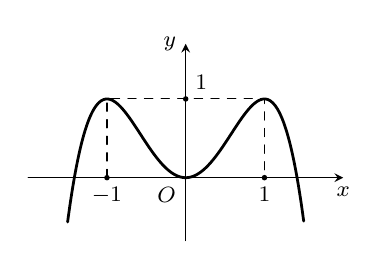
\begin{tikzpicture}[line join = round, line cap = round,>=stealth,font=\footnotesize,scale=1]
			
			\def \xmin{-2};
			\def \xmax{2};
			\def \ymin{-0.8};
			\def \ymax{1.7};
			\draw[->] (\xmin,0) -- (\xmax,0) node[below] {$x$};
			\draw[->] (0,\ymin) -- (0,0) node[below left] {$O$} -- (0,\ymax) node[left] {$y$};
			\clip (\xmin+0.1,\ymin+0.1) rectangle (\xmax-0.1,\ymax-0.1);
			\draw[smooth, line width=1,samples=100] plot[domain=-1.5:1.5] (\x,{-(\x)^4+2*(\x)^2});
			\draw[dashed] (-1,0) node[below] {$-1$} -- (-1,1) -- (1,1) -- (1,0) node[below] {$1$};
			\foreach \y in {1}
			{
				\fill (0,\y) circle (1pt);
			}
			\foreach \x in {-1,1}
			{
				\fill (\x,0) circle (1pt);
			}
			\draw (0,1) node[above right] {$1$};
		\end{tikzpicture}
	}
	\loigiai
	{
		\immini
		{
			Số nghiệm thực của phương trình $2f(x)=1\Leftrightarrow f(x)=\dfrac{1}{2}$ bằng số giao điểm của hai đồ thị $y=f(x)$ và $y=\dfrac{1}{2}$.\\
			Quan sát hình vẽ bên ta thấy hai đồ thị hàm số $y=f(x)$ và $y=\dfrac{1}{2}$ cắt nhau tại $4$ điểm phân biệt nên phương trình $2f(x)=1$ có $4$ nghiệm phân biệt.
		}
		{
			\begin{tikzpicture}[line join = round, line cap = round,>=stealth,font=\footnotesize,scale=1]
				
				\def \xmin{-2};
				\def \xmax{2.5};
				\def \ymin{-0.8};
				\def \ymax{1.7};
				\draw[->] (\xmin,0) -- (\xmax,0) node[below] {$x$};
				\draw[->] (0,\ymin) -- (0,0) node[below left] {$O$} -- (0,\ymax) node[left] {$y$};
				\clip (\xmin+0.1,\ymin+0.1) rectangle (\xmax-0.1,\ymax-0.1);
				\draw[smooth, line width=1,samples=100] plot[domain=-1.5:1.5] (\x,{-(\x)^4+2*(\x)^2});
				\draw[dashed] (-1,0) node[below] {$-1$} -- (-1,1) -- (1,1) -- (1,0) node[below] {$1$};
				\foreach \y in {1}
				{
					\fill (0,\y) circle (1pt);
				}
				\foreach \x in {-1,1}
				{
					\fill (\x,0) circle (1pt);
				}
				\draw (0,1) node[above right] {$1$};
				\draw (-2,0.5) -- (2,0.5) node[above] {$y=\dfrac{1}{2}$};
			\end{tikzpicture}
		}
	}
\end{ex}

\begin{ex}%[Đề thi thử THPT Kiến Thuỵ - Thái Bình]%[Bùi Mạnh Tiến, dự án 12EX-6]%[2D3B1-2]
	Họ nguyên hàm của hàm số $f(x)=\dfrac{x}{\sqrt{x^2+1}}$ là
	\choice
	{$2\sqrt{x^2+1}+C$}
	{$\dfrac{1}{\sqrt{x^2+1}}+C$}
	{$\dfrac{1}{2}\sqrt{x^2+1}+C$}
	{\True $\sqrt{x^2+1}+C$}
	\loigiai
	{
		Ta có $\displaystyle\int f(x) \mathrm{\,d}x=\displaystyle\int \dfrac{x}{\sqrt{x^2+1}} \mathrm{\,d}x=\dfrac{1}{2}\displaystyle\int \dfrac{\mathrm{\,d}\left(x^2+1\right)}{\sqrt{x^2+1}}=\dfrac{1}{2}\cdot 2\sqrt{x^2+1}+C=\sqrt{x^2+1}+C$.
	}
\end{ex}

\begin{ex}%[Đề thi thử THPT Kiến Thuỵ - Thái Bình]%[Bùi Mạnh Tiến, dự án 12EX-6]%[2H1B3-2]
	Cho hình chóp tứ giác đều $S.ABCD$ có tất cả các cạnh bằng $a$. Thể tích của khối chóp $S.ABC$ bằng
	\choice
	{\True $\dfrac{a^3\sqrt{2}}{12}$}
	{$\dfrac{a^3\sqrt{2}}{6}$}
	{$\dfrac{a^3\sqrt{2}}{4}$}
	{$\dfrac{a^3\sqrt{2}}{2}$}
	\loigiai
	{
		\immini
		{
			Gọi $O$ là tâm của hình vuông $ABCD$, vì $S.ABCD$ là hình chóp đều nên $SO\perp (ABCD)$.\\
			Ta có $AC=\sqrt{AB^2+BC^2}=\sqrt{a^2+a^2}=a\sqrt{2}\Rightarrow OA=OC=\dfrac{AC}{2}=\dfrac{a\sqrt{2}}{2}$.\\
			Tam giác vuông $SOA$ có $SO=\sqrt{SA^2-OA^2}=\sqrt{a^2-\dfrac{a^2}{2}}=\dfrac{a\sqrt{2}}{2}$.\\
			Thể tích khối chóp $S.ABC$ là
			\begin{align*}
				V_{S.ABC}=\dfrac{1}{3}SO\cdot S_{ABC}=\dfrac{1}{3}SO\cdot \dfrac{1}{2}AB\cdot BC=\dfrac{a^3\sqrt{2}}{12}.
			\end{align*}
		}
		{
			\begin{tikzpicture}[line join = round, line cap = round,>=stealth,font=\footnotesize,scale=0.8]
				\def \h{4};
				\path 
				(0,0) coordinate (A)
				(-1.5,-1.5) coordinate (B)
				(4,0) coordinate (D)
				($(B)+(D)-(A)$) coordinate (C)
				($(A)!0.5!(C)$) coordinate (O)
				($(O)+(0,\h)$) coordinate (S)
				;
				\draw (S) -- (B) -- (C) -- (D) -- (S) -- (C);
				\draw[dashed] (S) -- (A) -- (B) (A) -- (D) (A) -- (C) (B) -- (D) (S) -- (O);
				\foreach \x/\g in {A/180,B/180,C/0,D/0,S/90,O/-90} \fill[black](\x) circle (1pt)+(\g:3mm) node{$\x$};
			\end{tikzpicture}
		}
	}
\end{ex}

\begin{ex}%[Đề thi thử THPT Kiến Thuỵ - Thái Bình]%[Bùi Mạnh Tiến, dự án 12EX-6]%[2D2B4-3]
	\immini
	{
		Cho các hàm số $y=\log_a x$ và $y=\log_b x$ có đồ thị như hình vẽ bên. Đường thẳng $x=6$ cắt trục hoành, đồ thị hàm số $y=\log_a x$, và $y=\log_b x$ lần lượt tại $A$, $B$ và $C$. Nếu $\dfrac{AC}{AB}=\log_2 3$ thì khẳng định nào sau đây là đúng? 
		\choice
		{$b^2=a^3$}
		{$b^3=a^2$}
		{\True $\log_2 b=\log_3 a$}
		{$\log_3 b=\log_2 a$}
	}
	{
		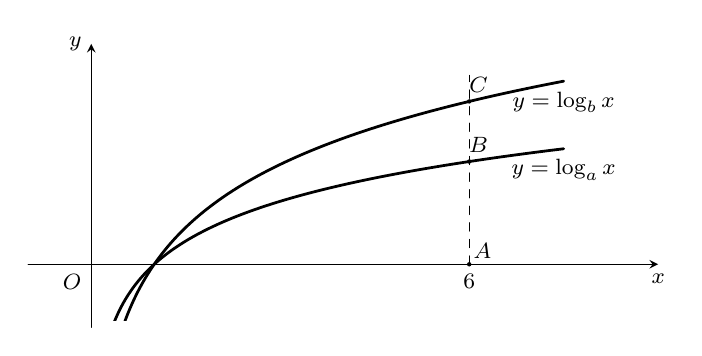
\begin{tikzpicture}[line join = round, line cap = round,>=stealth,font=\footnotesize,scale=0.8]
			\pgfmathsetmacro{\a}{3};
			\pgfmathsetmacro{\b}{2^(ln(\a)/ln(3))};
			\pgfmathsetmacro{\yB}{ln(6)/(ln(\a))};
			\pgfmathsetmacro{\yC}{ln(6)/(ln(\b))};
			\def \xmin{-1};
			\def \xmax{9};
			\def \ymin{-1};
			\def \ymax{3.5};
			\path
			(6,0) coordinate (A)
			(6,\yB) coordinate (B)
			(6,\yC) coordinate (C)
			;
			\draw[->] (\xmin,0) -- (\xmax,0) node[below] {$x$};
			\draw[->] (0,\ymin) -- (0,0) node[below left] {$O$} -- (0,\ymax) node[left] {$y$};
			\clip (\xmin+0.1,\ymin+0.1) rectangle (\xmax-0.1,\ymax-0.1);
			\draw[smooth, line width=1,samples=100] plot[domain=0.3:7.5] (\x,{ln(\x)/ln(\a)}) node[below] {$y=\log_a x$};
			\draw[smooth, line width=1,samples=100] plot[domain=0.3:7.5] (\x,{ln(\x)/ln(\b)}) node[below] {$y=\log_b x$};
			\draw[dashed] (6,0) node[below] {$6$} -- (6,3);
			\foreach \x/\g in {A/45,B/60,C/60} \fill[black](\x) circle (1pt)+(\g:3mm) node{$\x$};
		\end{tikzpicture}
	}
	\loigiai
	{
		Ta có $\dfrac{AC}{AB}=\log_2 3\Leftrightarrow \dfrac{\log_b 6}{\log_a 6}=\log_2 3\Leftrightarrow \dfrac{\log_6 a}{\log_6 b}=\log_2 3\Leftrightarrow \dfrac{\log_6 3\log_3 a}{\log_6 2\log_2 b}=\log_2 3\Leftrightarrow \log_3 a=\log_2 b$ $\left(\text{do }\dfrac{\log_6 3}{\log_6 2}=\log_2 3\right)$.	
	}
\end{ex}

\begin{ex}%[Đề thi thử THPT Kiến Thuỵ - Thái Bình]%[Bùi Mạnh Tiến, dự án 12EX-6]%[1D2K5-2]
	Một hộp chứa $16$ quả cầu gồm $8$ quả cầu màu xanh đánh số từ $1$ đến $8$ và $8$ quả cầu màu đỏ đánh số từ $9$ đến $16$. Lấy ngẫu nhiên $3$ quả cầu từ hộp đã cho. Xác suất để lấy được $3$ quả cầu có đủ hai màu đồng thời tích của các số ghi trên chúng là số chẵn bằng
	\choice
	{\True $\dfrac{5}{7}$}
	{$\dfrac{2}{7}$}
	{$\dfrac{3}{28}$}
	{$\dfrac{25}{28}$}
	\loigiai
	{
		Gọi không gian mẫu $\Omega$ là \lq\lq tập hợp tất cả các cách lấy ra $3$ quả cầu từ $16$ quả cầu\rq\rq, suy ra $n\left(\Omega\right)=\mathrm{C}_{16}^3=560$.\\
		Gọi $A$ là biến cố \lq\lq lấy được ba quả cầu có đủ $2$ màu và tích của các số ghi trên chúng là số chẵn\rq\rq. 
		\begin{itemize}
			\item Số cách chọn ra $3$ quả cầu có đủ $2$ màu là lấy ra $2$ quả cầu xanh, $1$ quả cầu đỏ hoặc lấy ra $1$ quả cầu xanh, $2$ quả cầu đỏ. Có $2\mathrm{C}_{8}^2\cdot \mathrm{C}_{8}^1$  cách.
			\item Ta chọn ra $3$ quả cầu có đủ $2$ màu nhưng tích các số ghi trên $3$ quả cầu là số lẻ. Khi đó ta cần chọn ra $2$ quả cầu xanh lẻ, $1$ quả cầu đỏ lẻ hoặc $1$ quả cầu xanh lẻ, $2$ quả cầu đỏ lẻ. Có $2\mathrm{C}_4^2\cdot \mathrm{C}_{4}^1$ cách chọn.
			\item Do đó số cách chọn ra $3$ quả cầu đủ $2$ màu nhưng tích các số ghi trên ba quả cầu đó là số chẵn là
			\begin{align*}
				2\mathrm{C}_{8}^2\cdot \mathrm{C}_{8}^1-2\mathrm{C}_{4}^2\cdot \mathrm{C}_{4}^1=400.
			\end{align*}
		\end{itemize}
		Suy ra $n\left(A\right)=400\Rightarrow \mathrm{P}(A)=\dfrac{n(A)}{n\left(\Omega\right)}=\dfrac{400}{560}=\dfrac{5}{7}$.
	}
\end{ex}

\begin{ex}%[Đề thi thử THPT Kiến Thuỵ - Thái Bình]%[Bùi Mạnh Tiến, dự án 12EX-6]%[1H3K3-3]
	Cho hình chóp $S.ABCD$ có đáy $ABCD$ là hình chữ nhật, $AB=a\sqrt{2}$, $AD=a$, $SA$ vuông góc
	với đáy và $SA=a$. Góc giữa $SC$ và $(SAB)$ bằng
	\choice
	{$90^\circ$}
	{$45^\circ$}
	{$60^\circ$}
	{\True $30^\circ$}
	\loigiai
	{
		\immini
		{
			Từ $\heva{& BC\perp AB \\ & BC\perp SA}\Rightarrow  BC\perp (SAB)$.\\
			Suy ra $SB$ là hình chiếu vuông góc của $SC$ lên $(SAB)$.\\
			Do đó $(SC,(SAB))=(SC,SB)=\widehat{CSB}$.\\
			Vì $CB\perp (SAB)\Rightarrow BC\perp SB$.
			Tam giác vuông $SBC$ có 
			\begin{align*}
				\tan \widehat{BSC}=\dfrac{BC}{SB}=\dfrac{AD}{\sqrt{SA^2+AB^2}}=\dfrac{a}{a\sqrt{3}}=\dfrac{\sqrt{3}}{3}\Rightarrow \widehat{BSC}=30^\circ.
			\end{align*}
			Do đó $(SC,(SAB))=30^\circ$.
		}
		{
			\begin{tikzpicture}[line join = round, line cap = round,>=stealth,font=\footnotesize,scale=1]
				\def \b{-1.4};
				\def \c{2.5};
				\def \h{3}
				\path
				(0,0) coordinate (A)
				(\b,\b) coordinate (B)
				(\c,\b) coordinate (C)
				($(A)+(C)-(B)$) coordinate (D)
				($(A)+(0,\h)$) coordinate (S)
				;
				\draw[dashed] (S) -- (A) -- (C) (A) -- (B) (A) -- (D) (A);
				\draw (S) -- (B) -- (C) -- (D) -- (S) -- (C);
				\foreach \x/\g in {A/180,B/180,C/0,D/0,S/90} \fill[black](\x) circle (1pt)+(\g:3mm) node{$\x$};
			\end{tikzpicture}
		}
	}
\end{ex}

\begin{ex}%[Đề thi thử THPT Kiến Thuỵ - Thái Bình]%[Bùi Mạnh Tiến, dự án 12EX-6]%[2D1K2-2]
	Cho hàm số bậc bốn $y=f(x)$ có bảng xét dấu của đạo hàm như hình vẽ.
	\begin{center}
		
\begin{tikzpicture}[line join = round, line cap = round,>=stealth,font=\footnotesize,scale=1]
			\tkzTabInit[nocadre=false,lgt=1.2,espcl=2.5,deltacl=0.6]
			{$x$ /0.6, $y'$ /0.6}
			{$-\infty$,$-1$,$1$,$3$,$+\infty$}
			\tkzTabLine{ ,+,$0$,-,$0$,+,$0$,-, }
		\end{tikzpicture}
	\end{center}
	Số điểm cực đại của hàm số $y=f\left(\sqrt{x^2-2x+2}\right)$ là
	\choice
	{$1$}
	{$4$}
	{\True $2$}
	{$3$}
	\loigiai
	{
		Ta có $y'=\left(\sqrt{x^2-2x+2}\right)'f'\left(\sqrt{x^2-2x+2}\right)=\dfrac{x-1}{\sqrt{x^2-2x+2}}f'\left(\sqrt{x^2-2x+2}\right)$.\\
		Phương trình $y'=0\Leftrightarrow \hoac{& x=1 \\ & f'\left(\sqrt{x^2-2x+2}\right)=0}\Leftrightarrow \hoac{& x=1 \\ & \sqrt{x^2-2x+2}=1\\& \sqrt{x^2-2x+2}=3}\Leftrightarrow \hoac{& x=1 \\ & (x-1)^2=0\\& x^2-2x-7=0}\Leftrightarrow \hoac{& x=1 \\ & x=1-2\sqrt{2}\\& x=1+2\sqrt{2}.}$\\
		Với $x=1$ là nghiệm bội lẻ của phương trình $y'=0$.\\
		Bảng xét dấu của hàm số $y'$ như sau
		\begin{center}
			
\begin{tikzpicture}[line join = round, line cap = round,>=stealth,font=\footnotesize,scale=1]
				\tkzTabInit[nocadre=false,lgt=1.2,espcl=2.5,deltacl=0.6]
				{$x$ /0.6, $y'$ /0.6}
				{$-\infty$,$1-2\sqrt{2}$,$1$,$1+2\sqrt{2}$,$+\infty$}
				\tkzTabLine{ ,+,$0$,-,$0$,+,$0$,-, }
			\end{tikzpicture}
		\end{center}	
		Hàm $y'$ đổi dấu từ dương sang âm tại qua điểm $x=1-2\sqrt{2}$ và $x=1+2\sqrt{2}$. Do đó số điểm cực đại của hàm số là $2$. 
	}
\end{ex}

\begin{ex}%[Đề thi thử THPT Kiến Thuỵ - Thái Bình]%[Bùi Mạnh Tiến, dự án 12EX-6]%[2D1K5-3]
	Cho hàm số bậc ba $y=f(x)$ có bảng biến thiên như sau
	\begin{center}
		
\begin{tikzpicture}[line join = round, line cap = round,>=stealth,font=\footnotesize,scale=1]
			\tkzTabInit[nocadre=false,lgt=1.2,espcl=2.5,deltacl=0.6]
			{$x$ /0.6, $f’(x)$ /0.6, $f(x)$ /2}
			{$-\infty$,$-1$,$1$,$+\infty$}
			\tkzTabLine{ ,+,$0$,-,$0$,+, }
			\tkzTabVar{-/$-\infty$,+/$4$,-/$0$,+/$+\infty$}
		\end{tikzpicture}
	\end{center}
	Tập hợp tất cả các số thực $m$ để phương trình $|f(x)+2|=m$ có $4$ nghiệm phân biệt trong đó có đúng một nghiệm dương là 
	\choice
	{$[2;4)$}
	{\True $[4;6)$}
	{$(2;6)$}
	{$(4;6)$}
	\loigiai
	{
		Đồ thị của hàm số đã cho là đồ thị của hàm số bậc ba nên nhận điểm uốn $U$ làm tâm đối xứng, suy ra $U(0;2)$. 
		Ta có bảng biến thiên như sau
		\begin{center}
			\begin{tikzpicture}[line join = round, line cap = round,>=stealth,font=\footnotesize,scale=1]
				\tkzTabInit[nocadre=false,lgt=2,espcl=2.5,deltacl=0.6]
				{$x$ /0.6, $f(x)+2$ /2, $|f(x)+2|$ /2}
				{$-\infty$,$-1$,$1$,$+\infty$}
				\tkzTabVar{-/$-\infty$,+/$6$,-/$2$,+/$+\infty$}
				\draw (N12)node[below](A) {$+\infty$};
				\draw ($(N22)!0.25!(N23)$) node (B) {$6$};
				\draw ($(N32)!0.85!(N33)$) node[above] (C) {$2$};
				\draw (N42) node[below] (D) {$+\infty$};
				\draw ($(N13)!0.5!(N23)$) node[above] (F) {$0$};
				\draw ($(B)!0.5!(C)$) node (G) {$4$};
				\draw[->] (A) -- (F);
				\draw[->] (F) -- (B);
				\draw[->] (B) -- (G);
				\draw[->] (G) -- (C);
				\draw[->] (C) -- (D);
				\path
				($(N12)!0.4!(N13)$) coordinate (d')
				($(N42)!0.4!(N43)$) coordinate (d)
				;
				\draw[red] (d') -- (d) node[below] {$y=m$};
				\draw[dashed] (G) -- ($(G)+(0,3.07)$) node[above] {$0$};
			\end{tikzpicture}
		\end{center}
		Dựa vào bảng biến thiên ta thấy phương trình $|f(x)+2|=m$ có $4$ nghiệm phân biệt trong đó có đúng một nghiệm dương khi và chỉ khi $4\leq m<6\Leftrightarrow m\in [4;6)$.
	}
\end{ex}

\begin{ex}%[Đề thi thử THPT Kiến Thuỵ - Thái Bình]%[Bùi Mạnh Tiến, dự án 12EX-6]%[2D2K6-3]
	Số nghiệm nguyên của bất phương trình $\left(9^x-5\cdot 6^x-6\cdot 4^x\right)\sqrt{128-2^{\sqrt{x}}}>0$ là
	\choice
	{$45$}
	{$48$}
	{$49$}
	{\True $44$}
	\loigiai
	{
		Điều kiện xác định $\heva{&x\geq 0\\& 128-2^{\sqrt{x}}\geq 0}\Leftrightarrow 0\leq x\leq 49.$
		Ta có 
		\begin{eqnarray*}
			\left(9^x-5\cdot 6^x-6\cdot 4^x\right)\sqrt{128-2^{\sqrt{x}}}>0&\Leftrightarrow& \heva{& 128-2^{\sqrt{x}}>0 \\ & 9^x-5\cdot 6^x-6\cdot 4^x>0}\\
			&\Leftrightarrow & \heva{& 2^{\sqrt{x}}<128=2^{7} \\ & \left[\left(\dfrac{3}{2}\right)^x\right]-5\left(\dfrac{3}{2}\right)^x-6>0}\\
			&\Leftrightarrow & \heva{& \hoac{& \left(\dfrac{3}{2}\right)^x>6\\&\left(\dfrac{3}{2}\right)^x<-1} \\ & x<49}\\
			&\Leftrightarrow &\heva{& \left(\dfrac{3}{2}\right)^x>6 \\ & x<49}\\
			&\Leftrightarrow &\heva{& x>\log_{\frac{3}{2}}6\approx 4{,}419 \\ & x<49.}
		\end{eqnarray*}
		Vì $x$ là số nguyên nên tập các giá trị của $x$ thoả mãn yêu cầu bài toán là $\{5;6;\ldots;48\}$.\\
		Có $48-5+1=44$ số nguyên $x$ thoả mãn yêu cầu bài toán.
	}
\end{ex}

\begin{ex}%[Đề thi thử THPT Kiến Thuỵ - Thái Bình]%[Bùi Mạnh Tiến, dự án 12EX-6]%[2D4K4-2]
	Trên tập hợp các số phức, xét phương trình $z^2-2(m+1)z+8m-4=0$ ($m$ là tham số thực). Có bao nhiêu giá trị nguyên của $m$ để phương trình đã cho có hai nghiệm phân biệt $z_1$, $z_2$ thoả mãn $\left|z_1^2-2mz_1+8m\right|=\left|z_2^2-2mz_2+8m\right|$?
	\choice
	{$5$}
	{$3$}
	{$6$}
	{\True $4$}
	\loigiai
	{
		Ta có $\Delta'=(m+1)^2-(8m-4)=m^2-6m+5$.\\
		Để phương trình có hai nghiệm phân biệt $z_1$, $z_2$ thì $\Delta'\neq 0\Leftrightarrow \heva{& m\neq 1 \\ & m\neq 5.}$\\
		Khi đó ta có $z_1^2-2(m+1)z_1+8m-4=z_2^2-2(m+1)z_2+8m-4=0\Leftrightarrow \heva{& z_1^2-2mz_1+8m=4+2z_1 \\ & z_2^2-2mz_2+8m=4+2z_2.}$\\
		Từ $\left|z_1^2-2mz_1+8m\right|=\left|z_2^2-2mz_2+8m\right|\Leftrightarrow \left|4+2z_1\right|=\left|4+2z_2\right|\Leftrightarrow |z_1+2|=|z_2+2|$.
		\begin{itemize}
			\item \textbf{Trường hợp $1$}: $\Delta'>0\Leftrightarrow \hoac{& m>5 \\ & m<1}$, khi đó $z_1$, $z_2$ là hai nghiệm thực của phương trình, do đó
			\begin{align*}
				|z_1+2|=|z_2+2|\Leftrightarrow \hoac{& z_1+2=z_2+2 \\ & z_1+2=-z_2-2}\Leftrightarrow \hoac{& z_1=z_2\text{ (vô lí)} \\ & z_1+z_2=-4}\Leftrightarrow 2(m+1)=-4\Leftrightarrow m=-3\text{ (thoả mãn).}
			\end{align*}
			\item \textbf{Trường hợp $2$}: $\Delta'<0\Leftrightarrow 1<m<5$. Khi đó phương trình có hai nghiệm $z_1$, $z_2$ thoả mãn
			\begin{align*}
				\hoac{& z_1=m+1-\sqrt{-\left(m^2-6m+5\right)}i \\ & z_2=m+1+\sqrt{-\left(m^2-6m+5\right)}i}
			\end{align*}
			Khi đó
			\begin{eqnarray*}
				&&|z_1+2|=|z_2+2|\\
				&\Leftrightarrow& \left|m+3-\sqrt{-\left(m^2-6m+5\right)}i\right|=\left|m+3+\sqrt{-\left(m^2-6m+5\right)}i\right|\\
				&\Leftrightarrow& (m+3)^2-\left(m^2-6m+5\right)=(m+3)^2-\left(m^2-6m+5\right)\text{ đúng với mọi }m \text{ thoả mãn }1<m<5.
			\end{eqnarray*}
			Vì $m\in \mathbb{Z}$ nên $m\in \{2;3;4\}$. \\
			Vậy $m\in \{-3;2;3;4\}$ có tất cả $4$ giá trị nguyên của $m$ thoả mãn yêu cầu bài toán.
		\end{itemize}	
	}
\end{ex}

\begin{ex}%[Đề thi thử THPT Kiến Thuỵ - Thái Bình]%[Bùi Mạnh Tiến, dự án 12EX-6]%[2H1K3-2]
	Cho hình chóp $S.ABC$ có $SA\perp (ABC)$, đáy là tam giác $ABC$ vuông tại $B$, $SA=a$, $AB=a\sqrt{2}$, góc tạo bởi hai mặt phẳng $(SAC)$ và $(SBC)$ là $60^\circ$. Tính theo $a$ thể tích khối chóp $S.ABC$.
	\choice
	{$\dfrac{a^3}{6}$}
	{$2a^3$}
	{\True $\dfrac{a^3\sqrt{3}}{3}$}
	{$\dfrac{2a^3\sqrt{3}}{3}$}
	\loigiai
	{
		\immini
		{
			Kẻ $BK\perp AC$, $BH\perp SC$.\\
			Từ $\heva{& BK\perp AC \\ & BK\perp SA}\Rightarrow BK\perp (SAC)\Rightarrow BK\perp SC$.\\
			Từ $\heva{& BH\perp SC \\ & BK\perp SC}\Rightarrow SC\perp (BHK)$.\\
			Do đó $((SAC),(SBC))=(BH,BK)=\widehat{BHK}\Rightarrow \widehat{BHK}=60^\circ$.\\
			Đặt $BC=x$. Ta có $SB=\sqrt{SA^2+AS^2}=a\sqrt{3}$.\\
			Ta có $BK=\dfrac{BA\cdot BC}{\sqrt{BA^2+BC^2}}=\dfrac{ax\sqrt{2}}{\sqrt{x^2+2a^2}}$, $BH=\dfrac{BS\cdot BC}{\sqrt{BS^2+BC^2}}=\dfrac{ax\sqrt{3}}{\sqrt{x^2+3a^2}}.$\\
			Tam giác $BHK$ có $\sin \widehat{BHK}=\dfrac{BK}{BH}\Leftrightarrow \dfrac{\sqrt{3}}{2}=\dfrac{\dfrac{ax\sqrt{2}}{\sqrt{x^2+2a^2}}}{\dfrac{ax\sqrt{3}}{\sqrt{x^2+3a^2}}}\Leftrightarrow x=a\sqrt{6}$.
		}
		{
			\begin{tikzpicture}[line join = round, line cap = round,>=stealth,font=\footnotesize,scale=1]
				\path 
				(0,0) coordinate (A)
				(1,-2) coordinate (B)
				(4,0) coordinate (C)
				(0,4) coordinate (S)
				($(S)!0.7!(C)$) coordinate (H)
				($(A)!0.3!(C)$) coordinate (K)
				;			
				\draw (S) -- (A) -- (B) -- (C) -- (S) -- (B) -- (H);
				\draw[dashed] (A) -- (C) (B) -- (K) -- (H);
				\foreach \x/\g in {S/90,A/180,B/-90,C/0,K/120,H/30} \fill[black](\x) circle (1pt)+(\g:3mm) node{$\x$};
				\tkzMarkRightAngles[](B,K,A S,A,C S,A,B B,H,C S,B,C)
			\end{tikzpicture}
			
		}
		\noindent
		Thể tích khối chóp $S.ABC$ là $V_{S.ABC}=\dfrac{1}{3}SA\cdot \dfrac{1}{2}BA\cdot BC=\dfrac{1}{3}\cdot a\cdot \dfrac{1}{2}\cdot a\sqrt{2}\cdot a\sqrt{6}=\dfrac{a^3\sqrt{3}}{3}$.
	}
\end{ex}

\begin{ex}%[Đề thi thử THPT Kiến Thuỵ - Thái Bình]%[Bùi Mạnh Tiến, dự án 12EX-6]%[2H3K3-2]
	Trong không gian với hệ tọa độ $Oxyz$, cho mặt phẳng $(P)\colon 2x-y+z-10=0$, điểm $I(1;3;2)$ và đường thẳng $d\colon \heva{& x=-2+2t \\ & y=1+t\\&z=1-t}$. Tìm phương trình đường thẳng $\Delta$ cắt $(P)$ và $d$ lần lượt tại hai điểm $M$ và $N$ sao cho $I$ là trung điểm của đoạn thẳng $MN$.
	\choice
	{\True $\dfrac{x+6}{7}=\dfrac{y+1}{4}=\dfrac{z-3}{-1}$}
	{$\dfrac{x+6}{7}=\dfrac{y+1}{-4}=\dfrac{z-3}{-1}$}
	{$\dfrac{x-6}{7}=\dfrac{y-1}{-4}=\dfrac{z-3}{-1}$}
	{$\dfrac{x-6}{7}=\dfrac{y-1}{4}=\dfrac{z+3}{-1}$}
	\loigiai
	{
		Vì $N\in d\Rightarrow N(-2+2t;1+t;1-t)$. Mà $I(1;3;2)$ là trung điểm của $MN$ suy ra
		\begin{align*}
			\heva{& x_M=2x_I-x_N=2\cdot 1-(-2+2t)=4-2t \\ & y_M=yx_I-y_N=2\cdot 3-(1+t)=5-t\\& z_M=2z_I-z_N=2\cdot 2-(1-t)=3+t}\Rightarrow M(4-2t;5-t;3+t).
		\end{align*}
		Vì $M\in (P)$ nên $2(4-2t)-(5-t)+(3+t)-10=0\Leftrightarrow t=-2\Rightarrow N(-6;-1;3)\Rightarrow \overrightarrow{NI}=(7;4;-1)$ là một véc-tơ chỉ phương của đường thẳng $\Delta$.\\
		Phương trình đường thẳng $\Delta$ đi qua $N(-6;-1;3)$ và nhận $\overrightarrow{NI}=(7;4;-1)$ làm véc-tơ chỉ phương là
		\begin{align*}
			\Delta \colon \dfrac{x+6}{7}=\dfrac{y+1}{4}=\dfrac{z-3}{-1}.
		\end{align*}
	}
\end{ex}

\begin{ex}%[Đề thi thử THPT Kiến Thuỵ - Thái Bình]%[Bùi Mạnh Tiến, dự án 12EX-6]%[1H3K5-4]
	Cho hình chóp $S.ABCD$ có đáy $ABCD$ là hình chữ nhật $AB=3a$, $AD=a$, $SA$ vuông góc với mặt phẳng đáy, $SA=2a$. Gọi $M$ là điểm thuộc đoạn thẳng $DC$ sao cho $DC=3DM$. Khoảng cách giữa hai đường $BM$ và $SD$ bằng
	\choice
	{$\dfrac{a\sqrt{6}}{3}$}
	{$\dfrac{2a}{3}$}
	{\True $\dfrac{a\sqrt{6}}{6}$}
	{$\dfrac{a}{3}$}
	\loigiai
	{
		\immini
		{
			Dựng hình bình hành $BMDN\Rightarrow DN\parallel BM$, $BN=DM=\dfrac{1}{3}DC=a\Rightarrow AN=AB-NB=2a$.\\
			Từ $DN\parallel BM\Rightarrow BM\parallel (SDN)\Rightarrow \mathrm{d}(SD,BM)=\mathrm{d}(BM,(SDN))=\mathrm{d}(B,(SDN))=\dfrac{1}{2}\mathrm{d}(A,(SDN))$.\\
			Kẻ $AK\perp DN$, $AH\perp SK$.\\
			Từ $\heva{& DN\perp AK \\ & SA\perp DN}\Rightarrow DN\perp (SAK)\Rightarrow DN\perp AH$.\\
			Từ $\heva{& AH\perp SK \\ & AH\perp DN}\Rightarrow AH\perp (SDN)\Rightarrow AH=\mathrm{d}(A,(SDN))$.
		}
		{
			\begin{tikzpicture}[line join = round, line cap = round,>=stealth,font=\footnotesize,scale=1]
				\def \b{-1.4};
				\def \c{2.5};
				\def \h{3}
				\path
				(0,0) coordinate (A)
				(\b,\b) coordinate (D)
				(\c,\b) coordinate (C)
				($(A)+(C)-(D)$) coordinate (B)
				($(A)+(0,\h)$) coordinate (S)
				($(D)!0.3333!(C)$) coordinate (M)
				($(B)!0.3333!(A)$) coordinate (N)
				($(D)!0.5!(N)$) coordinate (K)
				($(S)!0.6!(K)$) coordinate (H)
				;
				\draw[dashed] (S) -- (A) -- (C) (A) -- (B) (A) -- (D) (B) -- (M) (D) -- (N) (A) -- (K) -- (S) (A) -- (H);
				\draw (S) -- (B) -- (C) -- (D) -- (S) -- (C);
				\foreach \x/\g in {A/180,B/0,C/0,D/180,S/90,M/-90,K/-70,H/20,N/90} \fill[black](\x) circle (1pt)+(\g:3mm) node{$\x$};
			\end{tikzpicture}
			
		}
		\noindent
		Ta có $\dfrac{1}{AH^2}=\dfrac{1}{AK^2}+\dfrac{1}{AS^2}=\dfrac{1}{AD^2}+\dfrac{1}{AN^2}+\dfrac{1}{AS^2}=\dfrac{3}{2a^2}\Rightarrow AH=\dfrac{a\sqrt{6}}{3}$.\\
		Do đó $\mathrm{d}(BM,SD)=\dfrac{1}{2}\mathrm{d}(A,(SBD))=\dfrac{1}{2}AH=\dfrac{a\sqrt{6}}{6}$.
	}
\end{ex}

\begin{ex}%[Đề thi thử THPT Kiến Thuỵ - Thái Bình]%[Bùi Mạnh Tiến, dự án 12EX-6]%[2H3K1-4]
	Trong không gian với hệ toạ độ $Oxyz$, cho mặt cầu $(S)\colon (x-1)^2+(y-1)^2+z^2=25$ và hai điểm $A(7;9;0)$, $B(0;8;0)$. Với $M$ là điểm bất kì thuộc mặt cầu $(S)$, giá trị nhỏ nhất của biểu thức $MA+2MB$ bằng
	\choice
	{$5\sqrt{2}$}
	{$\dfrac{5\sqrt{5}}{2}$}
	{\True $5\sqrt{5}$}
	{$10$}
	\loigiai
	{
		\immini{Mặt cầu $(S)$ có tâm là $I(1;1;0)$, bán kính $R=5$.\\
			Ta có $IA=10=2R$.\\
			Gọi $E$ là trung điểm của $IA$, lấy điểm $N$ là trung điểm của $IE$. Dễ thấy $N\left(\dfrac{5}{2};3;0\right)$.\\
			Tam giác $IMA$ và $\triangle INM$ có $\widehat{I}$ chung và $\dfrac{IN}{IM}=\dfrac{IM}{IA}=\dfrac{1}{2}\Rightarrow\triangle IMA\backsim \triangle INM$.\\
			Suy ra $\dfrac{MA}{MN}=\dfrac{IM}{IN}=2\Leftrightarrow MA=2MN$.
		}
		{
			\begin{tikzpicture}[>=stealth,line join=round,line cap=round,font=\footnotesize,scale=0.7]
				\path (0,0) coordinate (I)
				(4,0) coordinate (A)
				(3,2.5) coordinate (B)
				($(I)!0.5!(A)$)coordinate (E)
				($(I)!0.5!(E)$)coordinate (N)
				($(I)+({2*cos (145)},{2*sin(145)})$) coordinate (M);
				;
				\draw (I)circle[radius=2];
				\draw (M)--(I)--(A)--(M)--(B)--(N)--(M);
				\foreach \p / \r in {A/-45,B/45,E/-45,N/-90,I/-135,M/135}
				\fill (\p) circle (1.2pt) node[shift={(\r:3mm)}]{$\p$};
		\end{tikzpicture}}
		\noindent
		Vậy ta có $P=MA+2MB=2MN+2MB=2(MN+MB)\ge2NB$. (vì $N$ và $B$ nằm hai phía đối với mặt cầu $(S)$)\\
		Dấu bằng xảy ra khi $M$ là điểm chung của đoạn thẳng $BN$ với mặt cầu $(S)$.\\
		Vậy giá trị nhỏ nhất của $P$ là $2NB=5\sqrt{5}$.
	}
\end{ex}

\begin{ex}%[Đề thi thử THPT Kiến Thuỵ - Thái Bình]%[Bùi Mạnh Tiến, dự án 12EX-6]%[2D1K1-2]
	\immini
	{
		Cho hàm số $f(x)$ và có đồ thị hàm số $f'(x)$ liên trục trên $\mathbb{R}$ như hình vẽ bên dưới. Có bao nhiêu giá trị nguyên của tham số $m\in (-10;10)$ để hàm số $y=f(2x-1)-2\ln \left(1+x^2\right)-2mx$ đồng biến trên khoảng $(-1;2)$?
		\choice
		{$6$}
		{\True $7$}
		{$5$}
		{$8$}
	}
	{
		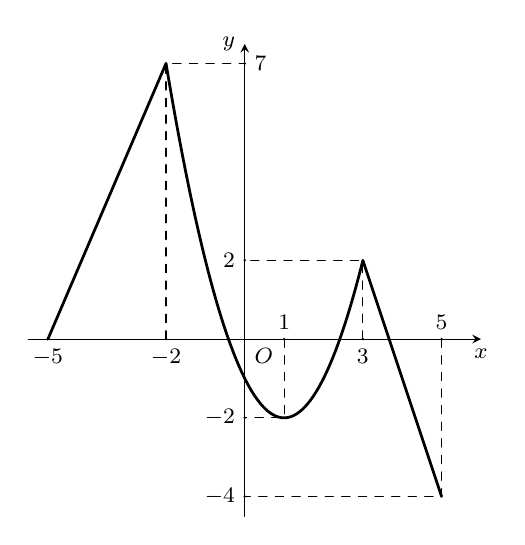
\begin{tikzpicture}[line join = round, line cap = round,>=stealth,font=\footnotesize,scale=0.5]
			\def \xmin{-5.5};
			\def \xmax{6};
			\def \ymin{-4.5};
			\def \ymax{7.5};
			\draw[->] (\xmin,0) -- (\xmax,0) node[below] {$x$};
			\draw[->] (0,\ymin) -- (0,0) node[below right] {$O$} -- (0,\ymax) node[left] {$y$};
			\clip (\xmin+0.1,\ymin+0.1) rectangle (\xmax-0.1,\ymax-0.1);
			\draw[smooth, line width=1,samples=100] plot[domain=-2:3] (\x,{(\x)^2-2*(\x)-1});
			\draw[line width=1] (-5,0) -- (-2,7) (3,2) -- (5,-4);
			\draw[dashed] (-2,0) node[below] {$-2$} -- (-2,7) -- (0,7) node[right] {$7$};
			\draw[dashed] (1,0) node[above] {$1$} -- (1,-2) -- (0,-2) node[left] {$-2$};
			\draw[dashed] (3,0) node[below] {$3$} -- (3,2) -- (0,2) node[left] {$2$};
			\draw[dashed] (5,0) node[above] {$5$} -- (5,-4) -- (0,-4) node[left] {$-4$};
			\foreach \y in {-4,-2,2,7}
			{
				\fill (0,\y) circle (1pt);
			}
			\foreach \x in {-5,-2,1,3,5}
			{
				\fill (\x,0) circle (1pt);
			}
			\draw (-5,0) node[below] {$-5$};
		\end{tikzpicture}
	}
	\loigiai
	{
		Ta có $y'=2\left[f'(2x-1)-\dfrac{2x}{x^2+1}-m\right]$.\\
		Hàm số đồng biến trên $(-1;2)$ khi
		\begin{eqnarray*}
			&&y'\geq 0,\text{ } \forall x\in (-1;2)\\
			&\Leftrightarrow & m\leq f'(2x-1)-\dfrac{2x}{x^2+1}=g(x),\text{ }\forall x\in (-1;2).
		\end{eqnarray*}
		Với $x\in (-1;2)\Rightarrow 2x-1\in (-3;3)\Rightarrow f'(2x-1)\geq -2$.\\
		Mà $-\dfrac{2x}{x^2+1}=\dfrac{(x-1)^2}{x^2+1}-1\geq -1$.\\
		Suy ra $g(x)\geq -2-1=-3$.\\
		Dấu \lq\lq =\rq\rq \text{} xảy ra khi và chỉ khi $x=1$.\\
		Vậy $\min\limits_{x \in (-1;2)} g(x)=-3$, do đó $m\leq -3$.\\
		Vì $m\in \mathbb{Z}$ và $m\in (-10;10)\Rightarrow m\in \{-9;-8;-7;-6;-5;-4;-3\}$.\\
		Có tất cả $7$ giá trị nguyên của $m$ thoả mãn yêu cầu bài toán.
	}
\end{ex}

\begin{ex}%[Đề thi thử THPT Kiến Thuỵ - Thái Bình]%[Bùi Mạnh Tiến, dự án 12EX-6]%[2D3K2-2]
	Cho hàm số $y=f(x)$ liên tục trên $\left[\dfrac{1}{3};3\right]$ thoả mãn $f(x)+x\cdot f\left(\dfrac{1}{x}\right)=x^3-x$, $\forall x\in \left[\dfrac{1}{3};3\right]$. 
	Giá trị của tích phân $I=\displaystyle\int\limits_{\frac{1}{3}}^{3} \dfrac{f(x)}{x^2+x} \mathrm{\,d}x$ bằng	
	\choice
	{\True $\dfrac{8}{9}$}
	{$\dfrac{3}{4}$}
	{$\dfrac{16}{9}$}
	{$\dfrac{2}{3}$}
	\loigiai
	{
		Đặt $t=\dfrac{1}{x}\Leftrightarrow x=\dfrac{1}{t}\Rightarrow  \mathrm{\,d}x=-\dfrac{1}{t^2}\mathrm{\,d}t$.\\
		Khi $x=\dfrac{1}{3}\Rightarrow t=3$, $x=3\Rightarrow t=\dfrac{1}{3}$.\\
		Khi đó $I=\displaystyle\int\limits_{3}^{\frac{1}{3}} \dfrac{f\left(\dfrac{1}{t}\right)}{\dfrac{1}{t^2}+\dfrac{1}{t}} \left(-\dfrac{1}{t^2}\right)\mathrm{\,d}t=\displaystyle\int\limits_{\frac{1}{3}}^{3} \dfrac{tf\left(\dfrac{1}{t}\right)}{t^2+t} \mathrm{\,d}t=\displaystyle\int\limits_{\frac{1}{3}}^{3} \dfrac{xf\left(\dfrac{1}{x}\right)}{x^2+x} \mathrm{\,d}x$.\\
		Suy ra $2I=\displaystyle\int\limits_{\frac{1}{3}}^{3} \dfrac{f(x)+xf\left(\dfrac{1}{x}\right)}{x^2+x} \mathrm{\,d}x=\displaystyle\int\limits_{\frac{1}{3}}^{3} \dfrac{x^3-x}{x^2+x} \mathrm{\,d}x=\displaystyle\int\limits_{\frac{1}{3}}^{3} (x-1) \mathrm{\,d}x=\left(\dfrac{x^2}{2}-x\right)\bigg|_{\frac{1}{3}}^3=\dfrac{16}{9}\Rightarrow I=\dfrac{8}{9}$.
	}
\end{ex}

\begin{ex}%[Đề thi thử THPT Kiến Thuỵ - Thái Bình]%[Bùi Mạnh Tiến, dự án 12EX-6]%[2H2K1-4]
	Một dụng cụ hình nón bằng thủy tinh, bên trong có chứa một lượng nước. Khi đặt dụng cụ sao cho đỉnh hình nón hướng xuống dưới theo chiều thẳng đứng thì phần không gian trống trong dụng cụ có chiều cao $2$ cm. Khi lật ngược dụng cụ để đỉnh hướng lên trên theo chiều thẳng đứng thì mực nước cao cách đỉnh của nón $8$ cm (hình vẽ minh họa bên dưới).
	\begin{center}
		\begin{tikzpicture}[line join = round, line cap = round,>=stealth,font=\footnotesize,scale=1]
			\def \x{2}%\bán kính trục lớn
			\def \y{0.4}%\bán kính trục nhỏ
			\def \xdaynho{1.5}%\bán kính trục lớn đáy nhỏ
			\def \ydaynho{0.3}%\bán kính trục nhỏ đáy nhỏ
			\def \xhai{6}%toạ độ hình thứ hai
			\def \h{4}%chiều cao hình nón
			\begin{scope}[shift={(0,0)}]
				\path
				(0,0) coordinate (S)
				($(S)+(0,\h)$) coordinate (O)
				($(O)+(-\x,0)$) coordinate (A)
				($(O)+(\x,0)$) coordinate (B)
				($(S)!0.75!(A)$) coordinate (A')
				($(S)!0.75!(B)$) coordinate (B')
				($(S)!0.75!(O)$) coordinate (O')
				;
				\draw (S) -- (A) (S) -- (B) -- (A);
				\draw[dashed] (A') -- (O');
				\draw (A) arc (180:0:\x cm and \y cm) arc (0:-180:\x cm and \y cm);
				\fill[color=gray,opacity=0.5] (A') arc (180:0:\xdaynho cm and \ydaynho cm) -- (S) -- (A');
				\draw[dashed] (A') arc (180:0:\xdaynho cm and \ydaynho cm);
				\draw (B') arc (0:-180:\xdaynho cm and \ydaynho cm);
				\draw[dashed] (S) -- (O);
				\path (O') -- (O) node[pos=0.45,right] {$2$ cm};
				\foreach \x/\g in {O/90,O'/0} \fill[black](\x) circle (1pt)+(\g:3mm) node{$\x$};
			\end{scope}
			\begin{scope}[shift={(\xhai,0)}]
				\path
				(0,\h) coordinate (S)
				($(S)+(0,-\h)$) coordinate (O)
				($(O)+(-\x,0)$) coordinate (A)
				($(O)+(\x,0)$) coordinate (B)
				($(S)!0.75!(A)$) coordinate (A')
				($(S)!0.75!(B)$) coordinate (B')
				($(S)!0.75!(O)$) coordinate (O')
				;
				\draw (S) -- (A) (S) -- (B);
				\draw[dashed] (A) -- (B) (A') -- (O');
				\draw[dashed] (A) arc (180:0:\x cm and \y cm);
				\draw (B) arc (0:-180:\x cm and \y cm);
				\fill[color=gray,opacity=0.5] (A') arc (180:0:\xdaynho cm and \ydaynho cm) -- (B) arc (0:-180:\x cm and \y cm) -- (A');
				\draw[dashed] (A') arc (180:0:\xdaynho cm and \ydaynho cm);
				\draw (B') arc (0:-180:\xdaynho cm and \ydaynho cm);
				\draw[dashed] (S) -- (O);
				\path (S) -- (O') node[pos=0.55,right] {$8$ cm};
				
			\end{scope}
			\foreach \x/\g in {O/-90,O'/0} \fill[black](\x) circle (1pt)+(\g:3mm) node{$\x$};
		\end{tikzpicture}
	\end{center}
	Biết chiều cao của nón là $h=a+\sqrt{b}$ cm, với $a$, $b$ là các số nguyên dương. Tính $T=a+b$.
	\choice
	{$22$}
	{$58$}
	{\True $86$}
	{$72$}
	\loigiai
	{
		Khi đỉnh nón hướng xuống dưới theo chiều thẳng đứng: $\dfrac{V_{\text{nước}}}{V_{\text{nón}}}=\left(\dfrac{h-2}{h}\right)^3\Rightarrow V_{\text{nước}}=\left(\dfrac{h-2}{h}\right)^3V_{\text{nón}}$.\\
		Khi lật ngược dụng cụ để đỉnh nón hướng lên trên: $\dfrac{V_{\text{nước}}}{V_{\text{nón}}}=1-\left(\dfrac{8}{h}\right)^3\Rightarrow V_{\text{nước}}=V_{\text{nón}}\left[1-\left(\dfrac{8}{h}\right)^3\right]$.\\
		Vì thể tích nước là không đổi nên ta có phương trình
		\begin{eqnarray*}
			&&\dfrac{(h-2)^3}{h^3}=1-\dfrac{8^3}{h^3}\\
			&\Leftrightarrow & (h-2)^3=h^3-8^3\\
			&\Leftrightarrow & 6h^2-12h-504=0\\
			&\Leftrightarrow &\hoac{& h=1+\sqrt{85} \text{ (thoả mãn)}\\ & h=1-\sqrt{85}<0.\text{ (không thoả mãn)}}
		\end{eqnarray*}
		Suy ra $a=1$, $b=85\Rightarrow a+b=86$.
	}
\end{ex}

\begin{ex}%[Đề thi thử THPT Kiến Thuỵ - Thái Bình]%[Bùi Mạnh Tiến, dự án 12EX-6]%[2D3K3-2]
	\immini
	{
		Một biển quảng cáo có dạng hình vuông $ABCD$ cạnh $AB = 4$ m. Trên tấm biển đó có các đường tròn tâm $A$ và đường tròn tâm $B$ cùng bán kính $R = 4$ m, hai đường tròn cắt nhau như hình vẽ. Chi phí để sơn phần gạch chéo là $150 000$ đồng/m$^2$, chi phí sơn phần màu đen là $100 000$ đồng/m$^2$, chi phí để sơn phần còn lại là $250 000$ đồng/m$^2$. Hỏi số tiền để sơn biển quảng cáo theo cách trên gần nhất với số tiền nào dưới đây?
		\choice
		{$3{,}017$ triệu đồng}
		{$1{,}213$ triệu đồng}
		{$2{,}06$ triệu đồng}
		{\True $2{,}195$ triệu đồng}
	}
	{
		\begin{tikzpicture}[line join = round, line cap = round,>=stealth,font=\footnotesize,scale=1]
			\pgfmathsetmacro{\so}{2*sqrt(3)}
			\path 
			(0,0) coordinate (A)
			(4,0) coordinate (B)
			(4,4) coordinate (C)
			(0,4) coordinate (D)
			(2,\so) coordinate (I)
			;
			\fill[pattern=north east lines] (A) arc (180:120:4 cm) arc (60:0:4 cm) -- (A);
			\fill[color=gray,opacity=0.5] (A) arc (180:120:4 cm) arc (60:90:4 cm) -- (A);
			\fill[color=gray,opacity=0.5] (B) arc (0:60:4 cm) arc (120:90:4 cm) -- (B); 
			\draw (A) -- (B) -- (C) -- (D) -- (A);
			\draw (B) arc (0:90:4 cm);
			\draw (A) arc (180:90:4 cm);
			\foreach \x/\g in {A/180,B/0,C/0,D/180} \fill[black](\x) circle (1pt)+(\g:3mm) node{$\x$};
			
		\end{tikzpicture}
	}
	\loigiai
	{
		\immini
		{
			Đặt hệ trục toạ độ $Oxy$ như hình vẽ.\\ 
			Đường tròn tâm $A$ bán kính $4$ có phương trình
			\begin{align*}
				x^2+y^2=16\Leftrightarrow y=\pm \sqrt{16-x^2}.
			\end{align*}
			Đường tròn tâm $B$ bán kính $4$ có phương trình
			\begin{align*}
				(x-4)^2+y^2=16\Leftrightarrow y=\pm \sqrt{16-(4-x)^2}=\pm \sqrt{8x-x^2}.
			\end{align*}
			Hoành độ điểm $I$ trên hình vẽ là nghiệm của phương trình
			\begin{align*}
				\sqrt{16-x^2}=\sqrt{8x-x^2}\Leftrightarrow 16-x^2=8x-x^2\Leftrightarrow x=2.
			\end{align*}
		}
		{
			\begin{tikzpicture}[line join = round, line cap = round,>=stealth,font=\footnotesize,scale=1]
				\pgfmathsetmacro{\so}{2*sqrt(3)}
				\path 
				(0,0) coordinate (A)
				(4,0) coordinate (B)
				(4,4) coordinate (C)
				(0,4) coordinate (D)
				(2,\so) coordinate (I)
				($(A)!1.2!(B)$) coordinate (x)
				($(A)!1.2!(D)$) coordinate (y)
				;
				\fill[pattern=north east lines] (A) arc (180:120:4 cm) arc (60:0:4 cm) -- (A);
				\fill[color=gray,opacity=0.5] (A) arc (180:120:4 cm) arc (60:90:4 cm) -- (A);
				\fill[color=gray,opacity=0.5] (B) arc (0:60:4 cm) arc (120:90:4 cm) -- (B); 
				\draw (A) -- (B) -- (C) -- (D) -- (A);
				\draw (B) arc (0:90:4 cm);
				\draw (A) arc (180:90:4 cm);
				\draw[->] (A) -- (x) node[below] {$x$};
				\draw[->] (A) -- (y) node[left] {$y$};
				\draw (A) node[left] {$A\equiv O$};
				\foreach \x/\g in {B/-90,I/90} \fill[black](\x) circle (1pt)+(\g:3mm) node{$\x$};
				
			\end{tikzpicture}
		}
		\noindent
		Số tiền cần dùng để sơn biển quảng cáo theo cách trên là
		\begin{align*}
			0{,}15\cdot 2\displaystyle\int\limits_{2}^{4} \sqrt{16-x^2} \mathrm{\,d}x+0{,}1\cdot 2\left(\dfrac{\pi \cdot 4^2}{4}-\displaystyle\int\limits_{2}^{4} 2\sqrt{16-x^2} \mathrm{\,d}x\right)+0{,}25\cdot \left[4^2-2\displaystyle\int\limits_{2}^{4} \sqrt{8x-x^2} \mathrm{\,d}x\right]\approx 2{,}19548\text{ triệu đồng}.
		\end{align*}
	}
\end{ex}

\begin{ex}%[Đề thi thử THPT Kiến Thuỵ - Thái Bình]%[Bùi Mạnh Tiến, dự án 12EX-6]%[2D2G5-5]
	Có bao nhiêu số nguyên dương $m$ để phương trình $\log_{\sqrt{3}}\left(x^3-6x^2+9x+1\right)+x(x-3)^2=3^m+2m-1$ có duy nhất một nghiệm thuộc khoảng $(-2;2)$?
	\choice
	{$0$}
	{$3$}
	{\True $1$}
	{$4$}
	\loigiai
	{
		Điều kiện xác định: $x^3-6x^2+9x+1>0\Leftrightarrow x>x_0$ với $x_0\approx -0{,}1038$ là nghiệm của phương trình $x_0^3-6x_0^2+9x_0+1=0$.\\
		Đặt $t=\log_3 \left(x^3-6x^2+9x+1\right)\Leftrightarrow x^3-6x^2+9x+1=3^t\Leftrightarrow x(x-3)^2=3^t-1$. Khi đó
		\begin{eqnarray*}
			&&\log_{\sqrt{3}}\left(x^3-6x^2+9x+1\right)+x(x-3)^2=3^m+2m-1\\
			&\Leftrightarrow& 2\log_3 \left(x^3-6x^2+9x+1\right)+x(x-3)^2=3^m+2m-1\\
			&\Leftrightarrow & 3^t+2t=3^m+2m.
		\end{eqnarray*}
		Xét hàm $f(u)=3^u+2u\Rightarrow f'(u)=3^u\ln 3+2>0$, $\forall u\in \mathbb{R}\Rightarrow f(u) $ là hàm đồng biến trên $\mathbb{R}$.\\
		Mà $f(t)=f(m)\Leftrightarrow m=t=\log_3 \left(x^3-6x^2+9x+1\right)$.\\
		Xét hàm số $g(x)=\log_3 \left(x^3-6x^2+9x+1\right)\Rightarrow g'(x)=\dfrac{3x^2-12x+9}{\left(x^3-6x^2+9x+1\right)\ln 3}$.\\
		Khi đó $g'(x)=0\Leftrightarrow 3x^2-12x+9=0\Leftrightarrow \hoac{& x=1\in (-2;2) \\ & x=3\notin (-2;2).}$\\
		Ta có bảng biến thiên của hàm số $g(x)$ trên $(x_0;2)$ như sau
		\begin{center}
			\begin{tikzpicture}[line join = round, line cap = round,>=stealth,font=\footnotesize,scale=1]
				\tkzTabInit[nocadre=false,lgt=1.2,espcl=2.5,deltacl=0.6]
				{$x$ /0.6, $g’(x)$ /0.6, $g(x)$ /2}
				{$x_0$,$1$,$2$}
				\tkzTabLine{ ,+,$0$,-, }
				%				\tkzTabVar{-/$-\infty$,+/$\log_3 5$,-/$1$}
				\draw (N13)
				node[above](A){$-\infty$};
				\draw (N22)
				node[below](B){$\log_3 5$};
				\path
				($(N32)!0.5!(N33)$) node(C) {$1$}
				;
				\draw[->] (A) -- (B);
				\draw[->] (B) -- (C);
			\end{tikzpicture}
		\end{center}
		Phương trình $m=g(x)$ có duy nhất một nghiệm thuộc khoảng $(-2;2)$ khi và chỉ khi $m=\log_3 5\notin \mathbb{Z}$ hoặc $m\leq 1$.\\
		Vì $m$ là số nguyên dương nên $m=1$.
	}
\end{ex}

\begin{ex}%[Đề thi thử THPT Kiến Thuỵ - Thái Bình]%[Bùi Mạnh Tiến, dự án 12EX-6]%[2D4G5-1]
	Gọi $S$ là tập hợp tất cả các số phức $z$ thoả mãn điều kiện $z\cdot \overline{z}=|z+\overline{z}|$. Xét các số phức $z_1$, $z_2\in S$ sao cho $|z_1-z_2|=1$. Giá trị nhỏ nhất của biểu thức $P=\left|z_1-\sqrt{3}i\right|+\left|\overline{z_2}+\sqrt{3}i\right|$ bằng 
	\choice
	{\True $2$}
	{$\sqrt{20-8\sqrt{3}}$}
	{$2\sqrt{3}$}
	{$1+\sqrt{3}$}
	\loigiai
	{
		\immini
		{
			Đặt $z=x+yi$ ($x$, $y\in \mathbb{R}$), suy ra $\overline{z}=x-yi$.\\
			Từ $z\cdot \overline{z}=\left|z+\overline{z}\right|\Leftrightarrow x^2+y^2=2|x|\Leftrightarrow \hoac{& (x-1)^2+y^2=1 \\ & (x+1)^2+y^2=1.}$\\
			Tập hợp điểm biểu diễn số phức $z$ là hai đường tròn tâm $I(1;0)$, bán kính $R=1$ và đường tròn $J(-1;0)$, bán kính $R=1$.\\
		}
		{
			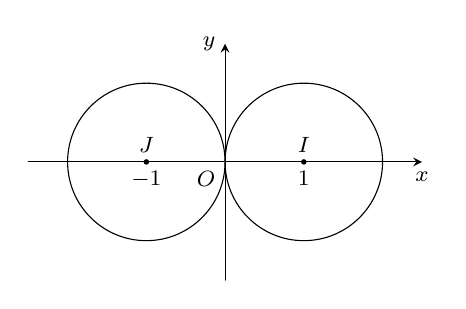
\begin{tikzpicture}[line join = round, line cap = round,>=stealth,font=\footnotesize,scale=1]
				\def \xmin{-2.5};
				\def \xmax{2.5};
				\def \ymin{-1.5};
				\def \ymax{1.5};
				\draw[->] (\xmin,0) -- (\xmax,0) node[below] {$x$};
				\draw[->] (0,\ymin) -- (0,0) node[below left] {$O$} -- (0,\ymax) node[left] {$y$};
				\clip (\xmin+0.1,\ymin+0.1) rectangle (\xmax-0.1,\ymax-0.1);
				\draw (1,0) circle (1cm);
				\draw (-1,0) circle (1cm);
				\fill (-1,0) circle (1pt) node[below] {$-1$};
				\fill (1,0) circle (1pt) node[below] {$1$};
				\draw (1,0) node[above] {$I$};
				\draw (-1,0) node[above] {$J$};  
			\end{tikzpicture}
		}
		\noindent
		Gọi $A\left(0;\sqrt{3}\right)$ và $M$, $N$ là hai điểm biểu diễn các số phức $z_1$, $z_2$. Ta có $AI=AJ=IJ=2\Rightarrow \triangle AIJ$ là tam giác đều cạnh bằng $2$.\\
		Ta có $P=\left|z_1-\sqrt{3}i\right|+\left|\overline{z_2}+\sqrt{3}i\right|=\left|z_1-\sqrt{3}i\right|+\left|z_2-\sqrt{3}i\right|=AM+AN$.
		\begin{itemize}
			\item \textbf{Trường hợp $1$}: $M$, $N$ cùng nằm trên $1$ đường tròn.
			\immini
			{
				Gọi $K$ là trung điểm của $MN$.\\
				Ta có $P=AM+AN>2AK\geq 2(IA-IK)>2(IA-R)=2(2-1)=2$.
			}
			{
				\begin{tikzpicture}[line join = round, line cap = round,>=stealth,font=\footnotesize,scale=1]
					\def \xmin{-2.5};
					\def \xmax{2.5};
					\def \ymin{-1.5};
					\def \ymax{2.5};
					\path 
					(0,1.732) coordinate (A)
					($(1,0)+(70:1)$) coordinate (M)
					($(1,0)+(130:1)$) coordinate (N)
					($(M)!0.5!(N)$) coordinate (K)
					;
					\draw[->] (\xmin,0) -- (\xmax,0) node[below] {$x$};
					\draw[->] (0,\ymin) -- (0,0) node[below left] {$O$} -- (0,\ymax) node[left] {$y$};
					\clip (\xmin+0.1,\ymin+0.1) rectangle (\xmax-0.1,\ymax-0.1);
					\draw (1,0) circle (1cm);
					\draw (-1,0) circle (1cm);
					\fill (-1,0) circle (1pt) node[below] {$J$};
					\fill (1,0) circle (1pt) node[below] {$I$}; 
					\draw (A) -- (M) -- (N) -- (A) -- (K) -- (1,0); 
					\foreach \x/\g in {A/180,N/180,M/70,K/-60} \fill[black](\x) circle (1pt)+(\g:3mm) node{$\x$};
					
				\end{tikzpicture}
			}
			\item \textbf{Trường hợp $2$}: $M$, $N$ nằm trên $2$ đường tròn.
			\immini
			{
				Ta có $P=AM+AN\geq AI-IM+AJ-JN=2-1+2-1=2$.\\
				Dấu \lq\lq =\rq\rq\text{} xảy ra khi và chỉ khi $A$, $N$, $J$ và $A$, $M$, $I$ thẳng hàng.\\
				Khi đó $M$, $N$ là trung điểm của $AI$, $AJ$ nên $MN$ là đường trung bình của $\triangle AIJ\Rightarrow MN=\dfrac{1}{2}IJ=1$.\\
				Vậy giá trị nhỏ nhất của $P$ là $2$.
			}
			{
				\begin{tikzpicture}[line join = round, line cap = round,>=stealth,font=\footnotesize,scale=1]
					\def \xmin{-2.5};
					\def \xmax{2.5};
					\def \ymin{-1.5};
					\def \ymax{2.2};
					\path 
					(0,1.732) coordinate (A)
					(1,0) coordinate (I)
					(-1,0) coordinate (J)
					($(I)+(130:1)$) coordinate (M)
					($(J)+(70:1)$) coordinate (N)
					($(M)!0.5!(N)$) coordinate (K)
					;
					\draw[->] (\xmin,0) -- (\xmax,0) node[below] {$x$};
					\draw[->] (0,\ymin) -- (0,0) node[below left] {$O$} -- (0,\ymax) node[left] {$y$};
					\clip (\xmin+0.1,\ymin+0.1) rectangle (\xmax-0.1,\ymax-0.1);
					\draw (1,0) circle (1cm);
					\draw (-1,0) circle (1cm);
					\fill (-1,0) circle (1pt) node[below] {$J$};
					\fill (1,0) circle (1pt) node[below] {$I$}; 
					\draw (A) -- (M) -- (N) -- (A) -- (I) (A) -- (J) -- (N) (I) -- (M); 
					\foreach \x/\g in {A/180,N/180,M/70} \fill[black](\x) circle (1pt)+(\g:3mm) node{$\x$};
					
				\end{tikzpicture}
			}
		\end{itemize}
	}
\end{ex}

\Closesolutionfile{ans}
\begin{indapan}{10}
	{ans/ans-2-TT-12-KienThuy-HaiPhong-23}
\end{indapan}